%COMANDO CHE DETERMINA IL TIPO DI DOCUMENTO CHE SI VUOLE CREARE

\documentclass[a4paper,12pt]{report}

%ELENCO DEI PACCHETTI UTILI PER LA STESURA DEL DOCUMENTO

\usepackage[utf8]{inputenc}
\usepackage[english, italian]{babel}
\usepackage{graphicx}
\usepackage{float}
\usepackage{tabularx}
\usepackage{makecell}
\usepackage{titlesec}
\usepackage{fancyhdr}
\usepackage{lastpage}
\usepackage{xurl}
\usepackage{hyperref}
\usepackage{geometry}
\usepackage[table,dvipsnames]{xcolor}
\setcounter{tocdepth}{5}
\setcounter{secnumdepth}{5}
\usepackage{caption}
\usepackage{etoolbox}% >= v2.1 2011-01-03
\usepackage{tikz}
\usepackage{listings}
\usepackage{scalerel}
\usepackage{longtable}
\usepackage{comment}
\usepackage{amssymb}
\usepackage{listings}

\titleformat{\chapter}[display]
{\normalfont\bfseries}{}{0pt}{\LARGE}

%COMANDO PER LA SPAZIATURA DEI TITOLI DAL BORDO DEL FOGLIO

\titlespacing*{\chapter}{0cm}{0cm}{0.2cm}

%COMANDO PER LA SPAZIATURA DEL TESTO DAI BORDI LATERALI

\geometry{
	left=20mm,
	right=20mm,
}

%COMADNO PER AVERE L'INDICE DEL NOME CHE SI VUOLE

\renewcommand{\contentsname}{Indice}

%COMADNI PER OTTENERE SUBSUBSECTION NUMERATE E PRESENTI NELL'INDICE

\setcounter{tocdepth}{5}
\setcounter{secnumdepth}{5}

%COMANDI PER OTTENERE HEADER E FOOTER

\pagestyle{plain}

\fancypagestyle{plain}{
	\fancyhf{}
	\lhead{
\includegraphics[width=3cm]{../../immagini/minilogo.jpg}}
	\chead{}
	\rhead{\fontsize{12}{10}Verbale Esterno 2021-04-15}
	\lfoot{}
	\cfoot{\thepage\ di \pageref{LastPage}}
	\rfoot{}
}

\pagestyle{plain}

%COMANDI PER LINK

\hypersetup{
	colorlinks=true,
	linkcolor=black,
	filecolor=black,
	urlcolor=blue,
	citecolor=black,
}

%COMANDI PER SNIPPET DI CODICE

\BeforeBeginEnvironment{lstlisting}{\begin{mdframed}\vspace{-0.7em}}
	\AfterEndEnvironment{lstlisting}{\vspace{-0.5em}\end{mdframed}}

% needed for \lstcapt
\def\ifempty#1{\def\temparg{#1}\ifx\temparg\empty}

% make new caption command for listings
\usepackage{caption}
\newcommand{\lstcapt}[2][]{%
	\ifempty{#1}%
	\captionof{lstlisting}{#2}%
	\else%
	\captionof{lstlisting}[#1]{#2}%
	\fi%
	\vspace{0.75\baselineskip}%
}

\definecolor{atomlightorange}{rgb}{0.88,0.76,0.55}
\definecolor{atomdarkgrey}{RGB}{59,62,75}

% set listings
\lstset{%
	basicstyle=\footnotesize\ttfamily\color{atomlightorange},
	framesep=20pt,
	belowskip=10pt,
	aboveskip=10pt
}

% add frame environment
\usepackage[%
framemethod=tikz,
skipbelow=8pt,
skipabove=13pt
]{mdframed}
\mdfsetup{%
	leftmargin=0pt,
	rightmargin=0pt,
	backgroundcolor=atomdarkgrey,
	middlelinecolor=atomdarkgrey,
	roundcorner=6
}

%BIBLIOGRAFIA

\makeatletter
\def\thebibliography#1{\chapter*{Bibliografia\@mkboth
		{Bibliografia}{Bibliografia}}\list
	{[\arabic{enumi}]}{\settowidth\labelwidth{[#1]}\leftmargin\labelwidth
		\advance\leftmargin\labelsep
		\usecounter{enumi}}
	\def\newblock{\hskip .11em plus .33em minus .07em}
	\sloppy\clubpenalty4000\widowpenalty4000
	\sfcode`\.=1000\relax}
\makeatother

%DEFINIZIONE COLORI

\definecolor{airforceblue}{rgb}{0.36, 0.54, 0.66}


\begin{document}
\makeatletter
\begin{titlepage}
	\begin{center}
		\vspace*{-5cm}
		\author{Jawa Druids} 
		\title{Norme di Progetto}
		\date{} %LASCIARE QUESTO CAMPO VUOTO, SE LO TOLGO STAMPA LA DATA CORRENTE
		
\includegraphics[width=0.5\linewidth]{../immagini/DRUIDSLOGO.jpg}\\[4ex]
		{\huge \bfseries  \@title }\\[2ex] 
		{\LARGE  \@author}\\[50ex]
		\vspace*{-9cm}
		\begin{table}[H]
			\renewcommand{\arraystretch}{1.4}
			\centering
			\begin{tabular}{r | l}
				\textbf{Versione} & 1.0.0 \\%RIGA PER INSERIRE LA VERSIONE ULTIMA DEL DOCUMENTO
				\textbf{Data approvazione} & 10-01-2021\\
				\textbf{Responsabile} & Igli Mezini \\
				\textbf{Redattori} & \makecell[tl]{Igli Mezini \\ Andrea Cecchin \\ Andrea Dorigo \\ Mattia Cocco \\ Alfredo Graziano} \\		
				\textbf{Verificatori} & \makecell[tl]{Margherita Mitillo \\ Andrea Dorigo \\ Emma Roveroni} \\
				%MAKECELL SERVE PER POI ANDARE A CAPO ALL'INTERNO DELLA CELLA
				\textbf{Stato} & Stato\\
				\textbf{Lista distribuzione} & \makecell[tl]{Jawa Druids \\ Prof. Tullio Vardanega \\ Prof. Riccardo Cardin}\\
				\textbf{Uso} & Interno     
			\end{tabular}
		\end{table}
		\vspace{0.1cm}
		\hfill \break
		\fontsize{17}{10}\textbf{Sommario} \\
		\vspace{0.1cm}
		Il documento redatto riferisce le regole, gli strumenti e le convenzioni a cui il gruppo JawaDruids ha stabilito di attenersi e seguire per l'intera durata dello sviluppo del progetto.
	\end{center}
\end{titlepage}
\makeatother
	\quad
\begin{center}
	\LARGE\textbf{Registro delle modifiche}
\end{center}
\def\tabularxcolumn#1{m{#1}}
{\rowcolors{2}{RawSienna!90!RawSienna!20}{RawSienna!70!RawSienna!40}

\begin{center}
	\renewcommand{\arraystretch}{1.4}
	\begin{longtable}{|p{4cm}|p{3cm}|p{2.8cm}|p{2cm}|p{1.7cm}|}
	\hline
	\rowcolor{airforceblue}
	\textbf{Modifica} & \textbf{Autore} & \textbf{Ruolo} & \textbf{Data} & \textbf{Versione}
	\\
	\hline
	\textit{Approvazione del documento per RR} & Igli Mezini & \textit{Responsabile} & 10-01-2021 & v1.0.0
	\\
	\hline
	\textit{Revisione Finale del documento} & Margherita Mitillo & \textit{Verificatore} & 09-01-2021 & v0.9.0
	\\
	\hline
	\textit{Verificato capitolo \S~\ref{Formazione}} & Margherita Mitillo & \textit{Verificatore} & 08-01-2021 & v0.8.0
	\\
	\hline
	\textit{Verificate sezioni \S~\ref{ProcessiPrimariProgettazione}, \S~\ref{ProcessiPrimariCodifica}, \S~\ref{ProcessiPrimariStrumenti}, \S~\ref{Standard ISO/IEC 15504} } & Andrea Dorigo & \textit{Verificatore} & 08-01-2021 & v0.7.0
	\\
	\hline
	\textit{Verificate sezioni \S~\ref{ProcessiDiSupportoGestioneDellaConfigurazione}, \S~\ref{ProcessiOrganizzativiProcessoDiPianificazione}, \S~\ref{ProcessiOrganizzativiFormazione}} & Margherita Mitillo & \textit{Verificatore} & 07-01-2021 & v0.6.0
	\\
	\hline
	\textit{Verificate sezioni \S~\ref{ProcessiDiSupportoVerifica}, \S~\ref{ProcessiDiSupportoValidazione}, \S~\ref{StandardISO/IEC9126}} & Emma Roveroni & \textit{Verificatore} & 07-01-2021 & v0.5.0
	\\
	\hline
	\textit{Aggiunto capitolo \S~\ref{Formazione}} & Mattia Cocco & \textit{Amministratore} & 06-01-2021 & v0.4.7
	\\
	\hline
	\textit{Aggiunte sezioni \S~\ref{ProcessiDiSupportoVerifica} e \S~\ref{ProcessiDiSupportoValidazione} } & Alfredo Graziano & \textit{Amministratore} & 05-01-2021 & v0.4.6
	\\
	\hline
	\textit{Aggiunto capitolo \S~\ref{ProcessiOrganizzativiFormazione}} & Mattia Cocco & \textit{Amministratore} & 05-01-2021 & v0.4.5
	\\
	\hline
	\textit{Aggiunte sezioni \S~\ref{ProcessiPrimariProgettazione}, \S~\ref{ProcessiPrimariCodifica}, \S~\ref{ProcessiPrimariStrumenti}} & Andrea Cecchin & \textit{Amministratore} & 03-01-2021 & v0.4.4
	\\
	\hline
	\textit{Aggiunta sezione \S~\ref{ProcessiDiSupportoGestioneDellaConfigurazione}} & Andrea Dorigo & \textit{Amministratore} & 02-01-2021 & v0.4.3
	\\
	\hline
	\textit{Aggiunte sezioni \S~\ref{ProcessiPrimariProspettiveAnalisiDeiRequisitiMetriche}, \S~\ref{ProcessiDiSupportoVerificaDescrizione}} & Mattia Cocco & \textit{Amministratore} & 02-01-2021 & v0.4.2
	\\
	\hline
	\textit{Aggiunto capitolo \S~\ref{Standard ISO/IEC 15504}} & Alfredo Graziano & \textit{Amministratore} & 01-01-2021 & v0.4.1
	\\
	\hline
	\textit{Verificate sezioni \S~\ref{ProcessiDiSupportoGestioneDellaQualità} e \S~\ref{ProcessiOrganizzativiProcessoDiCoordinamento} } & Emma Roveroni & \textit{Verificatore} & 31-12-2020 & v0.4.0
	\\
	\hline
	\textit{Aggiunta sezione \S~\ref{ProcessiOrganizzativiProcessoDiPianificazioneMetriche}} & Alfredo Graziano & \textit{Amministratore} & 30-12-2020 & v0.3.4
	\\
	\hline
	\textit{Aggiunte sezioni \S~\ref{ProcessiDiSupportoGestioneDellaQualità}, \S~\ref{StandardISO/IEC9126} } & Mattia Cocco & \textit{Amministratore} & 30-12-2020 & v0.3.3
	\\
	\hline
	\textit{Aggiunte sezioni \S~\ref{ProcessiOrganizzativiProcessoDiPianificazioneScopo}, \S~\ref{ProcessiOrganizzativiProcessoDiPianificazioneRuoliDiProgetto}, \S~\ref{ProcessiOrganizzativiProcessoDiPianificazioneAssegnazioneDeiCompiti}, \S~\ref{ProcessiOrganizzativiProcessoDiPianificazioneTrelloEGitkraken}, \S~\ref{ProcessiOrganizzativiProcessoDiPianificazioneStrumenti} } & Igli Mezini & \textit{Amministratore} & 30-12-2020 & v0.3.2
	\\
	\hline
	\textit{Aggiunte sezioni \S~\ref{ProcessiOrganizzativiProcessoDiCoordinamentoScopo}, \S~\ref{ProcessiOrganizzativiProcessoDiCoordinamentoComunicazione}, \S~\ref{ProcessiOrganizzativiProcessoDiCoordinamentoRiunioni}, \S~\ref{ProcessiOrganizzativiProcessoDiCoordinamentoStrumentiUtilizzatiPerIlProcessoDiCoordinamento} } & Igli Mezini & \textit{Amministratore} & 29-12-2020 & v0.3.1
	\\
	\hline
	\textit{Verificata sezione \S~\ref{ProcessiDiSupportoDocumentazione}} & Andrea Dorigo & \textit{Verificatore} & 15-12-2020 & v0.3.0
	\\
	\hline
	\textit{Verificate sezioni \S~\ref{ProcessiPrimariFornitura} e \S~\ref{ProcessiPrimariSviluppo} } & Margherita Mitillo & \textit{Verificatore} & 11-12-2020 & v0.2.0
	\\
	\hline
	\textit{Verificato capitolo \S~\ref{Introduzione}} & Margherita Mitillo & \textit{Verificatore} & 10-12-2020 & v0.1.0
	\\
	\hline
	\textit{Aggiunte sezioni \S~\ref{ProcessiDiSupportoDocumentazioneMetricheCorrettezzaOrtografica}, \S~\ref{ProcessiDiSupportoDocumentazioneDirectoryDiUnDocumento}} & Andrea Dorigo & \textit{Amministratore} & 08-12-2020 & v0.0.9
	\\
	\hline
	\textit{Aggiunte sezioni \S~\ref{ProcessiDiSupportoDocumentazioneMetriche}, \S~\ref{ProcessiDiSupportoDocumentazioneStrumentiDiStesura}} & Igli Mezini & \textit{Amministratore} & 03-12-2020 & v0.0.8
	\\
	\hline
	\textit{Aggiunte sezioni \S~\ref{ProcessiDiSupportoDocumentazioneStrutturaGeneraleDeiDocumenti}, \S~\ref{ProcessiDiSupportoDocumentazioneNormeTipografiche}, \S~\ref{ProcessiDiSupportoDocumentazioneElementiGrafici}} & Igli Mezini & \textit{Amministratore} & 01-12-2020 & v0.0.7
	\\
	\hline
	\textit{Aggiunta sezione \S~\ref{ProcessiPrimariSviluppo}} & Andrea Cecchin & \textit{Amministratore} & 30-11-2020 & v0.0.6
	\\
	\hline
	\textit{Aggiunte sezioni \S~\ref{ProcessiDiSupportoDocumentazioneTemplateInFormatoLatex}, \S~\ref{ProcessiDiSupportoDocumentazioneDocumentiProdotti}, \S~\ref{ProcessiDiSupportoDocumentazioneDirectoryDiUnDocumento}} & Igli Mezini & \textit{Amministratore} & 29-11-2020 & v0.0.5
	\\
	\hline
	\textit{Aggiunte sezioni \S~\ref{ProcessiDiSupportoDocumentazioneDescrizione}, \S~\ref{ProcessiDiSupportoDocumentazioneImplementazioneDelDocumento}, \S~\ref{ProcessiDiSupportoDocumentazioneCicloDiVitaDiUnDocumento}} & Igli Mezini & \textit{Amministratore} & 28-11-2020 & v0.0.4
	\\
	\hline
	\textit{Aggiunte sezioni \S~\ref{ProcessiPrimariFornituraStudioDiFattibilità}, \S~\ref{ProcessiPrimariFornituraAltraDocumentazioneDaFornire}, \S~\ref{ProcessiPrimariFornituraStrumenti}} & Andrea Cecchin & \textit{Amministratore} & 26-11-2020 & v0.0.3
	\\
	\hline
	\textit{Aggiunte sezioni \S~\ref{Introduzione} e \S~\ref{ProcessiPrimariFornituraScopo}} & Andrea Cecchin & \textit{Amministratore} & 25-11-2020 & v0.0.2
	\\
	\hline
	\textit{Prima stesura del documento} & Andrea Cecchin & \textit{Amministratore} & 24-11-2020 & v0.0.1
	\\
	\hline
	\end{longtable}
\end{center}


	\tableofcontents{}
	\listoffigures
	\chapter{Introduzione}\label{Introduzione}

\section{Scopo del documento}
Il Piano di Qualifica è un documento su cui si prevede di operare per l’intera durata del progetto 
e il cui scopo è presentare e descrivere le strategie di verifica e validazione adottate 
dal gruppo Jawa Druids al fine di garantire la qualità di prodotto e di processo.  
Per raggiungere questo obbiettivo viene applicato un sistema di verifica continua sui processi in corso e 
sulle attività svolte, in modo da rilevare e correggere subito eventuali anomalie, riducendo lo spreco di risorse 
ed il rischio di reiterare gli stessi errori.
\section{Scopo del prodotto}
L'obiettivo del prodotto \textit{GDP - Gathering Detection Platform} di \textit{Sync Lab} è la creazione di un sistema software in 
grado di acquisire, monitorare, utilizzare e correlare tra loro tutti i dati acquisiti tramite sensoristica (come telecamere di videosorveglianza)
e altre sorgenti dati (es. orari con il maggior numero di visite degli esercizi commerciali estrapolati da Google) con lo
scopo di avere indicazioni di potenziali assembramenti e quindi di fornire supporto per trovare soluzioni che limitino tali condizioni.
\section{Glossario}
Al fine di favorire la comprensione totale della documentazione relativa al progetto, viene fornito un documento denominato \textit{Glossario -- fornire versione}
che riporta la spiegazione della terminologia specifica e tecnica utilizzata per la stesura di questo ed altri documenti.
Tali termini, quando utilizzati, vengono contrassegnati con un apice \textsuperscript{G} alla fine della parola.
\section{Standard di progetto}
Decidere se scrivere di aver utilizzato un determinato standard ISO per il software, se si, definirlo nelle norme di progetto!
\section{Riferimenti}
\subsection{Riferimenti normativi}
\begin{itemize}
	\item \textit{Norme di Progetto}
\end{itemize}
\subsection{Riferimenti informativi}
\begin{itemize}
	\item \textit{IEEE Recommended Practice for Software Requirements Specifications:}\\
	\url{https://ieeexplore.ieee.org/document/720574}
	\item \textit{Seminario per approfondimenti tecnici del capitolato C3:}\\
	\url{https://www.math.unipd.it/~tullio/IS-1/2020/Progetto/ST1.pdf}		
\end{itemize}
	\chapter{Processi Primari}\label{ProcessiPrimari}
\section{Fornitura}\label{ProcessiPrimariFornitura}
\subsection{Scopo}\label{ProcessiPrimariFornituraScopo}
La fornitura secondo lo standard ISO/IEC 12207:1995 descrive le attività$_G$ e i compiti svolti dal fornitore al fine di sviluppare un prodotto soddisfacente e che rispetti appieno le richieste del committente$_G$.
Durante questa fase si prevede la compilazione di diversi documenti, i quali verranno inviati al committente$_{\scaleto{G}{3pt}}$ per guadagnare la possibilità di lavorare al progetto offerto dall'azienda \textit{Sync Lab}.
Il fornitore esegue un'attività$_{\scaleto{G}{3pt}}$ di analisi e stesura dello \textit{Studio di Fattibilità}, documento che rileva i rischi e le criticità riscontrate nella richiesta di appalto.
Si definisce inoltre un accordo contrattuale con il proponente$_G$ mediante il quale si regolano i rapporti con l'azienda, la consegna e la manutenzione del prodotto sviluppato. 

\subsection{Studio di Fattibilità}\label{ProcessiPrimariFornituraStudioDiFattibilità}
Lo \textit{Studio di Fattibilità} consiste nell'analisi e nella valutazione sistematica delle caratteristiche, dei costi, e dei possibili risultati di un progetto sulla base di una preliminare idea di massima.
A seguito della presentazione dei capitolati d'appalto da parte di ogni proponente$_{\scaleto{G}{3pt}}$ avvenuta il 05-11-2020, il \textit{Responsabile di Progetto} si è impegnato a programmare incontri con tutti i componenti del gruppo \textit{Jawa Druids} per valutare le scelte di ogni membro e attuare così un primo scambio di idee. Una volta individuato il capitolato d'interesse gli \textit{Analisti} hanno provveduto alla stesura dello \textit{Studio di Fattibilità}, i quali hanno fornito un'analisi accurata dei capitolati presentati.
Nella stesura dello \textit{Studio di Fattibilità} per ogni capitolato$_{\scaleto{G}{3pt}}$ si riporterà:
\begin{itemize}
	\item informazioni generali: informazioni riguardanti il proponente$_{\scaleto{G}{3pt}}$;
	\item descrizione del capitolato$_{\scaleto{G}{3pt}}$: sintesi del progetto da sviluppare; 
	\item finalità del progetto: finalità richieste dal capitolato$_{\scaleto{G}{3pt}}$ d'appalto;
	\item tecnologie interessate: tecnologie che verranno utilizzate nello svolgimento del capitolato$_{\scaleto{G}{3pt}}$
	\item aspetti positivi: aspetti favorevoli alla scelta del capitolato$_{\scaleto{G}{3pt}}$;
	\item criticità e fattori di rischio: problematiche che potrebbero sorgere durante lo svolgimento del capitolato;
	\item conclusioni: accettazione o rifiuto del capitolato$_{\scaleto{G}{3pt}}$ in base alle informazioni illustrate precedentemente e anche all'interesse dimostrato da ogni membro nel gruppo.
\end{itemize}
\subsection{Altra documentazione da fornire}\label{ProcessiPrimariFornituraAltraDocumentazioneDaFornire}
Oltre allo \textit{Studio di Fattibilità} vengono consegnati altri documenti all'azienda \textit{Sync Lab} ed ai committenti \textit{Prof. Tullio Vardanega} e \textit{Prof. Riccardo Cardin}. Questi documenti sono necessari al fine di tracciare le attività$_{\scaleto{G}{3pt}}$ di Analisi, Pianificazione, Verifica, Validazione e Controllo di Qualità per assicurare una completa trasparenza durante tutta la durata del ciclo di vita del progetto.
I documenti in questione sono:
\begin{itemize}
	\item \textit{Analisi dei Requisiti}: identifica e dettaglia in modo completo ed esaustivo i requisiti$_G$ del sistema descritto nel capitolato che il fornitore si impegna a soddisfare;
	\item \textit{Piano di Qualifica}: illustra la strategia complessiva di verifica e validazione proposta dal fornitore per pervenire al collaudo del sistema con la massima efficienza ed efficacia;
	\item \textit{Piano di Progetto}: presenta l'organigramma dettagliato del fornitore, lo schema proposto per l'assegnazione e la rotazione dei ruoli di progetto, l'impegno complessivo previsto per ogni ruolo e per ogni individuo, l'analisi dei rischi, la pianificazione di massima per la realizzazione del prodotto, e il corrispondente conto economico preventivo.
\end{itemize} 
Alla documentazione appena illustrata il gruppo \textit{Jawa Druids} allegherà inoltre una lettera di presentazione con la quale si formalizza l'impegno nel portare al termine il capitolato prescelto entro i termini definiti nella lettera e rispettandone i requisiti$_{\scaleto{G}{3pt}}$ minimi.
\subsection{Strumenti}\label{ProcessiPrimariFornituraStrumenti}
Di seguito sono riportati gli strumenti impiegati dal gruppo durante il progetto per il processo di fornitura.
\subsubsection{Documenti Google}\label{ProcessiPrimariFornituraStrumentiDocumentiGoogle}
Questo strumento viene utilizzato per la realizzazione di documenti in cui più persone possono lavorarci contemporaneamente osservando le modifiche in tempo reale. 
\begin{center}
	\url{https://docs.google.com}
\end{center}
\subsubsection{Fogli Google}\label{ProcessiPrimariFornituraStrumentiFogliGoogle}
Questo strumento viene utilizzato per la realizzazione di grafici e fogli di calcolo in cui più persone possono lavorarci contemporaneamente osservando le modifiche in tempo reale.
\begin{center}
	\url{https://www.google.com/sheets}
\end{center}


\section{Sviluppo}\label{ProcessiPrimariSviluppo}
\subsection{Scopo}\label{ProcessiPrimariScopo}
Il processo di sviluppo contiene tutte le attività$_{\scaleto{G}{3pt}}$ che riguardano la produzione del software richiesto dal cliente, in particolare analisi dei requisiti$_{\scaleto{G}{3pt}}$, design, codifica, integrazione, test e installazione.
\subsection{Descrizione}\label{ProcessiPrimariDescrizione}
Di seguito vengono elencate le varie attività$_{\scaleto{G}{3pt}}$ che caratterizzano tale processo:
\begin{itemize}
	\item Analisi dei requisiti$_{\scaleto{G}{3pt}}$;
	\item Progettazione architetturale;
	\item Codifica del software.
\end{itemize}
\subsection{Prospettive}\label{ProcessiPrimariProspettive}
Le prospettive alla fine della stesura del processo in questione sono le seguenti:
\begin{itemize}
	\item individuare e stabilire gli obbiettivi di sviluppo;
	\item individuare e stabilire i vincoli tecnologici;
	\item individuare e stabilire i vincoli di design;
	\item produrre un prodotto finale che rispecchi gli obiettivi imposti nello sviluppo e che superi i test e i controlli di qualità stabiliti dal proponente$_{\scaleto{G}{3pt}}$.
\end{itemize}
\subsubsection{Analisi dei requisiti}\label{ProcessiPrimariProspettiveAnalisiDeiRequisiti}
\paragraph{Scopo}\label{ProcessiPrimariProspettiveAnalisiDeiRequisitiScopo}\mbox{}\\
L'analisi dei requisiti$_{\scaleto{G}{3pt}}$ viene redatto dagli \textit{Analisti}, lo scopo è quello di definire le funzionalità che il nuovo prodotto deve offrire, ovvero i requisiti$_{\scaleto{G}{3pt}}$ che devono essere soddisfatti dal software sviluppato.\\
Gli obiettivi della stesura dell'\textit{Analisi dei Requisiti} sono:
\begin{itemize}
	\item stabilire lo scopo nello sviluppo del prodotto;
	\item definire riferimenti precisi ed affidabili ai \textit{Progettisti};
	\item stabilire i requisiti$_{\scaleto{G}{3pt}}$ e le funzionalità concordate con il cliente;
	\item individuare per i \textit{Verificatori} riferimenti per le attività$_{\scaleto{G}{3pt}}$ di controllo dei test.
\end{itemize}
\paragraph{Descrizione}\label{ProcessiPrimariProspettiveAnalisiDeiRequisitiDescrizione}\mbox{}\\
I requisiti$_{\scaleto{G}{3pt}}$ possono essere individuati in diverse fonti, quali:
\begin{itemize}
	\item \textit{Capitolato$_{\scaleto{G}{3pt}}$ d'Appalto}: i requisiti$_{\scaleto{G}{3pt}}$ sono stati individuati attraverso la lettura del documento fornito dal proponente$_{\scaleto{G}{3pt}}$ \textit{Sync Lab} sul capitolato proposto;
	\item \textit{Verbali Interni}: attraverso le riunioni attuate internamente dagli \textit{Analisti} sono emersi vari requisiti$_{\scaleto{G}{3pt}}$;
	\item \textit{Verbali Esterni}: attraverso contatti e discussioni effettuate con il responsabile aziendale Fabio Pallaro sono emersi requisiti$_{\scaleto{G}{3pt}}$, i quali vi sarà assegnato un codice presente nella tabella dei tracciamenti;
\end{itemize}
\paragraph{Prospettive}\label{ProcessiPrimariProspettiveAnalisiDeiRequisitiProspettive}\mbox{}\\
L'obiettivo dell'\textit{Analisi dei Requisti} è quello di redigere un documento che racchiuda al suo interno tutti i requisiti$_{\scaleto{G}{3pt}}$ richiesti dal proponente$_{\scaleto{G}{3pt}}$.
\paragraph{Struttura}\label{ProcessiPrimariProspettiveAnalisiDeiRequisitiStruttura}\mbox{}\\ %wip non è ancora perfettamente definito ???
L'\textit{Analisi dei requisiti$_{\scaleto{G}{3pt}}$} è strutturato nel seguente modo:
\begin{itemize}
	\item \textbf{Introduzione}: in questa sezione si introduce lo scopo del documento e riferimenti a documenti esterni;
	\item \textbf{Descrizione generale}: il prodotto viene descritto, si individuano le fasi generali del progetto e l'utenza a cui è destinato il prodotto;
	\item \textbf{Fasi del prodotto}: si elencano in gruppi le fasi del progetto, le quali vengono suddivise in parti per individuare più dettagliatamente tutti i processi di sviluppo del software;
	\item \textbf{Requisiti$_{\scaleto{G}{3pt}}$}: utilizzando le fasi descritte e tutti i documenti sopra indicati si dettagliano tutti i requisiti$_{\scaleto{G}{3pt}}$ obbligatori, facoltativi e desiderabili da implementare.
\end{itemize}
\paragraph{Classificazione dei requisiti}\label{ProcessiPrimariProspettiveAnalisiDeiRequisitiClassificazioneDeiRequisiti}\mbox{}\\% RS1.2 = rs(requisiti specifici) 1(fase generale a cui si riferiscono) 2(numero del requisito incrementale)
I requisiti$_{\scaleto{G}{3pt}}$ sono stati individuati utilizzando la seguente codifica:
\begin{center}
	\textbf{RS[classificazione][tipo\_di\_requisito][codice\_requisito]}
\end{center} 
La descrizione della classificazione è la seguente:
\begin{itemize}
	\item \textbf{RS}: è l'acronimo per Requisito$_{\scaleto{G}{3pt}}$ Specifico;
	\item \textbf{Classificazione}: individua la classificazione del requisito$_{\scaleto{G}{3pt}}$:
	\begin{itemize}
		\item Funzionale: indicato dalla lettera "F";
		\item Qualità: indicato dalla lettera "Q";
		\item Vincolo: indicato dalla lettera "V";
		\item Prestazionale: indicato dalla lettera "P".
	\end{itemize}
	\item \textbf{Tipo\_di\_requisito$_{\scaleto{G}{3pt}}$}: individua la tipologia di requisito$_{\scaleto{G}{3pt}}$:
	\begin{itemize}
		\item Obbligatorio: indicato con la lettera "O" individua un requisito$_{\scaleto{G}{3pt}}$ essenziale allo sviluppo del progetto e necessario al suo completamento;
		\item Desiderabile: indicato con la lettera "D" individua un requisito$_{\scaleto{G}{3pt}}$ utile al prodotto e che dà valore aggiunto ad esso, ma non essenziale al suo completamento;
		\item Facoltativo: indicato con la lettera "F" individua un requisito$_{\scaleto{G}{3pt}}$ che può essere sviluppato, ma può anche non essere completato;
	\end{itemize}
	\item \textbf{Codice\_requisito}: è rappresentato da un codice identificativo univoco nella forma gerarchica padre/figlio.
\end{itemize}
Ogni requisito$_{\scaleto{G}{3pt}}$ è strutturato nella tabella nel seguente modo:
\begin{itemize}
	\item \textbf{Identificativo}: individua univocamente il requisito$_{\scaleto{G}{3pt}}$;
	\item \textbf{Descrizione}: descrizione del requisito$_{\scaleto{G}{3pt}}$ richiesto nella determinata fase;
	\item \textbf{Tipo di requisito$_{\scaleto{G}{3pt}}$}: individua la tipologia di requisito$_{\scaleto{G}{3pt}}$ obbligatorio, desiderabile e facoltativo;
	\item \textbf{Fonte}: ogni requisito$_{\scaleto{G}{3pt}}$ è ricavato da una delle seguenti fonti:
	\begin{itemize}
		\item Capitolato$_{\scaleto{G}{3pt}}$: individua il documento del capitolato$_{\scaleto{G}{3pt}}$;
		\item Interno: il requisito$_{\scaleto{G}{3pt}}$ è stato individuato dagli analisti;
		\item Verbale: si tratta del documento in riferimento alla discussione con il proponente$_{\scaleto{G}{3pt}}$;
		\item Fasi del capitolato$_{\scaleto{G}{3pt}}$: il requisito$_{\scaleto{G}{3pt}}$ è stato individuato dalla fase del capitolato$_{\scaleto{G}{3pt}}$ individuata con il proprio codice.
	\end{itemize}
\end{itemize}
\paragraph{Classificazione delle fasi}\label{ProcessiPrimariProspettiveAnalisiDeiRequisitiClassificazioneDelleFasi}\mbox{}\\% FC1.2 = fc(fasi capitolato) 1 (macro-fase) 2(fase precisa)
La descrizione dettagliata delle fasi è stata incorporata nel documento per individuare la fase in cui il requisito$_{\scaleto{G}{3pt}}$ è necessario che venga implementato o sia possibile l'implementazione.\\
La classificazione delle fasi è definita nel seguente modo:
\begin{center}
	\textbf{FC[codice\_macro-fase].[codice\_fase]}
\end{center}
La descrizione della classificazione è la seguente:
\begin{itemize}
	\item \textbf{FC}: è l'acronimo per Fasi Capitolato$_{\scaleto{G}{3pt}}$;
	\item \textbf{Codice\_macro-fase}: individua un numero riferito alla fase dello sviluppo del progetto;
	\item \textbf{Codice\_fase}: individua un numero riferito ad una suddivisione della fase del progetto.
\end{itemize}
Ogni suddivisione delle fasi è strutturato nel seguente modo:
\begin{itemize}
	\item \textbf{Principali}:
	\begin{itemize}
		\item \textbf{Identificativo}: inserito prima del nome della fase per individuarla univocamente;
		\item \textbf{Nome}: identifica il nome della fase;
		\item \textbf{Descrizione}: descrizione dello scopo della fase in analisi.
	\end{itemize}
	\item \textbf{Aggiuntivi}:
\begin{itemize}
	\item \textbf{Input}: dati in ingresso necessari allo sviluppo della fase;
	\item \textbf{Output}: dati in uscita elaborati o modificati durante la fase;
	\item \textbf{Linguaggio di programmazione}: linguaggio di programmazione utilizzato per lo sviluppo della fase;
	\item \textbf{Processo}: sono le operazioni svolte nella fase;
	\item \textbf{Risposta ad errori}: operazione della fase nel caso di errori;
	\item \textbf{Tipi di algoritmi}: individua gli algoritmi utilizzabili;
	\item \textbf{Strumenti}: sono strumenti utilizzati nello svolgimento della fase;
	\item \textbf{Vincolo}: vincoli individuati dal gruppo o dal proponente$_{\scaleto{G}{3pt}}$.
\end{itemize}
\end{itemize}
\paragraph{Qualità dei requisiti}\label{ProcessiPrimariProspettiveAnalisiDeiRequisitiQualitàDeiRequisiti}\mbox{}\\
Ogni requisito$_{\scaleto{G}{3pt}}$ deve rispettare le seguenti qualità:
\begin{itemize}
	\item devono essere correttamente descritti;
	\item non devono essere ambigui, ogni requisito$_{\scaleto{G}{3pt}}$ fornirà un'unica interpretazione;
	\item devono essere completi, cioè descrivere in modo completo e in tutte le sue parti la funzionalità da implementare;
	\item ogni requisito$_{\scaleto{G}{3pt}}$ deve essere consistente, cioè non deve avere conflitti con altri requisiti$_{\scaleto{G}{3pt}}$ individuati;
	\item devono essere modificabili, cioè ogni requisito$_{\scaleto{G}{3pt}}$ nel corso dello sviluppo del progetto può essere rivalutato e modificato e bisogna mantenere uno storico dei cambiamenti;
	\item ogni requisito$_{\scaleto{G}{3pt}}$ deve essere tracciabile, cioè ogni requisito$_{\scaleto{G}{3pt}}$ deve essere tracciabile ad ogni suo test o codice di implementazione o alla sua origine;
	\item ogni requisito$_{\scaleto{G}{3pt}}$ deve essere classificato per importanza o stabilità;
	\item ogni requisito$_{\scaleto{G}{3pt}}$ deve essere verificabile, cioè deve essere possibile una sua verifica attraverso un processo nel quale una persona o una macchina può controllarlo.
\end{itemize}

\paragraph{Metriche}\label{ProcessiPrimariProspettiveAnalisiDeiRequisitiMetriche}\mbox{}\\
Con \textbf{MQPD01} si intende la \textbf{Totalità delle implementazioni}. Indice riportante l'interezza del prodotto software, rispetto ai requisiti$_{\scaleto{G}{3pt}}$ posti, mediante un valore percentuale.:

\begin{center}
	\textbf{T=($1-\frac{RnI}{RI}$)*100}
\end{center}
Dove:
\begin{itemize}
	\item \textbf{T} sta per \textit{Totalità}, riferito ai requisiti$_{\scaleto{G}{3pt}}$ da implementare;
	\item \textbf{RnI} sta per \textit{Requisito$_{\scaleto{G}{3pt}}$ non Implementato};
	\item \textbf{RI} sta per \textit{Requisito$_{\scaleto{G}{3pt}}$ Implementato}.
\end{itemize}
I range accettabili per il risultato di \textbf{T} sono così suddivisi:
\begin{itemize}
	\item 90\% $<$ \textbf{T} $\leq$ 100\% indica che la copertura dei requisiti$_{\scaleto{G}{3pt}}$ proposti è quasi totale;
	\item 80\% $<$ \textbf{T} $\leq$ 90\% indica che la copertura dei requisiti$_{\scaleto{G}{3pt}}$ proposti è sufficiente, buona;
	\item \textbf{T} $\leq$ 80\% indica che la copertura dei requisiti$_{\scaleto{G}{3pt}}$ proposti è insufficiente.
\end{itemize}


\subsection{Progettazione}\label{ProcessiPrimariProgettazione}
\subsubsection{Scopo}\label{ProcessiPrimariProgettazioneScopo}
La Progettazione è un'attività$_{\scaleto{G}{3pt}}$ svolta dai \textit{Progettisti}. In questa fase si individuano, attraverso l'\textit{Analisi dei Requisiti}, le caratteristiche che il prodotto deve avere per soddisfare tutti i requisiti$_{\scaleto{G}{3pt}}$ richiesti dal proponente$_{\scaleto{G}{3pt}}$. Lo scopo è quello di determinare la soluzione migliore per risolvere ogni requisito$_{\scaleto{G}{3pt}}$ individuato. 
\subsubsection{Aspettative}\label{ProcessiPrimariProgettazioneAspettative}
Alla conclusione della stesura della progettazione si ha come risultato la realizzazione dell'architettura del software da sviluppare. Tale architettura è necessaria ai programmatori per individuare le istruzioni necessarie a sviluppare il prodotto finito.
\subsubsection{Descrizione}\label{ProcessiPrimariProgettazioneDescrizione}
La progettazione è suddivisa principalmente in due parti:
\begin{itemize}
	\item \textbf{Technology baseline$_G$}: contiene tutte le specifiche adottate nella progettazione ad alto livello e delle sue componenti, i test di verifica e l'elenco dei diagrammi UML$_G$ utilizzati per la definizione dell'architettura;
	\item \textbf{Product baseline$_G$}: perfeziona ulteriormente la fase di progettazione, integrando ciò che è riportato nella technology baseline$_{\scaleto{G}{3pt}}$, definendo inoltre i test necessari alla verifica.
\end{itemize}

\subsubsection{Technology baseline}\label{ProcessiPrimariProgettazioneTecnologyBaseline}
La technology baseline$_{\scaleto{G}{3pt}}$ viene redatta dal \textit{Progettista} ed include:
\begin{itemize}
	\item \textbf{Diagramma UML$_{\scaleto{G}{3pt}}$}: diagrammi sulle classi usate, package, attività$_{\scaleto{G}{3pt}}$ e sequenze;
	\item \textbf{Tecnologie}: descrizione delle tecnologie utilizzate nel progetto, i loro vantaggi e svantaggi;
	\item \textbf{Design pattern}: descrizione di ogni design pattern per la realizzazione dell'architettura, ognuno di essi viene accompagnato da un diagramma che ne espone il significato e la struttura; 
	\item \textbf{Tracciamento delle componenti}: ogni componente viene riferito al requisito$_{\scaleto{G}{3pt}}$ che soddisfa;
	\item \textbf{Test di integrazione}: corrispondono a tutti i test necessari alla verifica del sistema in tutte le sue unità.
\end{itemize}
\subsubsection{Product baseline}\label{ProcessiPrimariProgettazioneProductBaseline}
La product baseline$_{\scaleto{G}{3pt}}$ viene redatta dal \textit{Progettista} ed include:
\begin{itemize}
	\item \textbf{definizioni delle classi e funzioni}: descrizione univoca delle classi e funzioni evitando ridondanze;
	\item \textbf{tracciamento}: ogni requisito$_{\scaleto{G}{3pt}}$ viene tracciato attraverso le classi e funzioni, questo è necessario per individuare se è stato soddisfatto il requisito$_{\scaleto{G}{3pt}}$;
	\item \textbf{test di unità}: definiscono test per la verifica delle funzionalità del prodotto.
\end{itemize}
\subsection{Codifica}\label{ProcessiPrimariCodifica}

\subsubsection{Scopo}\label{ProcessiPrimariCodificaScopo}
La fase di codifica è la scrittura del codice per sviluppare la miglior soluzione del prodotto. In questa sezione si introdurranno tutte le norme necessarie allo sviluppo di un codice uniformato tra tutti i \textit{Programmatori} e rispettoso delle regole standard indicate nel documento.
\subsubsection{Aspettative}\label{ProcessiPrimariCodificaAspettative}
Conclusa la fase di codifica ci si attende un codice pulito e facile da leggere, utile nelle successive validazioni, modifiche e per agevolare la sua manutenzione. L'obiettivo è quello di sviluppare un prodotto conforme alle richieste individuate con il proponente$_{\scaleto{G}{3pt}}$. 

\subsubsection{Descrizione}\label{ProcessiPrimariCodificaDescrizione}
In questa fase la programmazione del prodotto dovrà rispettare le norme descritte nel documento. Perseguendo gli obiettivi individuati nel documento \textit{Piano di qualifica v1.0.0} si produrrà un software con un'alta qualità di codice.

\subsubsection{Stile di codifica}\label{ProcessiPrimariCodificaStileDiCodifica}
All'interno di questo paragrafo vengono elencate le norme da rispettare da ogni membro del gruppo per raggiungere uniformità del codice:

\begin{itemize}
	\item \textbf{Indentazione}: ogni blocco di codice scritto per il prodotto da sviluppare deve essere ben indentato e deve rispettare una misura di 4 spazi (equivalenti alla pressione del tasto \textit{tab}). Fanno eccezione a questa regola i commenti che vengono inseriti per spiegazioni di blocchi di codice;
	\item \textbf{Parentesizzazione}: le parentesi devono essere utilizzate in linea col blocco di codice scritto e non in una linea sottostante per separarlo;
	\item \textbf{Univocità delle variabili, metodi e funzioni}: ogni variabile, metodo e funzione utilizzata deve avere un nome significativo, esplicativo ed univoco;
	\item \textbf{Classi}: ogni classe deve avere il proprio nome scritto con l'iniziale maiuscola;
	\item \textbf{Metodi e funzioni}: il nome di metodi e funzioni devono iniziare per lettera minuscola e se composti da più parole le successive devono essere scritte con lettera maiuscola (stile \textit{CamelCase});
	\item \textbf{Lingua}: i commenti devono essere scritti in lingua inglese.
\end{itemize}

\subsection{Strumenti}\label{ProcessiPrimariStrumenti}

\subsubsection{PragmaDB}\label{ProcessiPrimariStrumentiPragmaDB}
Programma utilizzato per il tracciamento dei requisiti$_{\scaleto{G}{3pt}}$.
\begin{center}
	\url{https://pragmadb.com/}
\end{center}
\subsubsection{StarUML}\label{ProcessiPrimariStrumentiDrawIo}
Questo strumento viene usato per la realizzazione di diagrammi UML$_{\scaleto{G}{3pt}}$ in quanto è stato ritenuto semplice da utilizzare.
\begin{center}
	\url{https://staruml.io/}
\end{center}
\subsubsection{Atom}\label{ProcessiPrimariStrumentiAtom}
Questo strumento viene usato per la codifica del linguaggio Java e Javascript. Offre la piena compatibilità con Linux, Windows, macOS e fornisce molte integrazioni aggiuntive.
\begin{center}
	\url{https://atom.io}
\end{center}
	\chapter{Processi Di Supporto}\label{ProcessiDiSupporto}
I processi di supporto sono documentazione, gestione della configurazione, gestione della qualità, verifica e validazione
\section{Documentazione}\label{3.1}
\subsection{Descrizione}\label{3.1.1}
Questa sezione fornisce le norme per la stesura, la verifica e l'approvazione dei documenti. Tali regole vanno seguite in tutti i documenti ufficiali prodotti durante il ciclo di vita del software, garantendo cosi la coerenza e la validità degli stessi
\subsection{Implementazione del documento}\label{3.1.2}
 Per ogni documento che si intende sviluppare è necessario identificare:
\begin{itemize}
\item \textbf {titolo o nome:} che sia significativo ed ufficiale;
	\item \textbf {scopo:} che espliciti il contenuto generale del documento e la sua funzionalità come 		documentazione di progetto;
		\item \textbf {destinatari:} che indichi i soggetti a cui il documento è destinato, o coloro i quali sono tenuti a prenderne visione;
			\item \textbf {procedure di gestione:} che guidino i responsabili nello sviluppo corretto e normato del documento, durante tutto il suo ciclo di vita;
				\item \textbf {versionamento:} pianificazione di versioni intermedie e finali del documento.
\end{itemize}
\subsection{Ciclo di vita di un documento}\label{3.1.3}
Ogni documento prodotto percorre le tappe del seguente ciclo di vita:
\begin{itemize}
\item \textbf{creazione:} il documento viene creato partendo da un template progettato a tale
	scopo, situato nella cartella Template del repository remoto;
	\item \textbf{strutturazione:} il documento viene fornito di un registro delle modifiche, di un indice dei   contenuti e, se necessario, di un indice delle figure e di un indice delle tabelle presenti nel corpo del documento;
		\item \textbf{stesura:} il corpo del documento viene scritto progressivamente, da più membri del gruppo, adottando un metodo incrementale;
			\item \textbf{revisione:} ogni singola sezione del corpo del documento viene regolarmente rivista da almeno un membro del gruppo, che deve essere obbligatoriamente diverso dal redattore della parte in verifica; se necessario, la verifica può essere svolta da più persone: in questo caso può partecipare anche chi ha scritto la sezione in verifica a patto che non si occupi della parte da esso redatta;
				\item \textbf{approvazione:} terminata la revisione, il Responsabile di Progetto stabilisce la validità del documento, che solo a questo punto può essere considerato completo e può essere quindi rilasciato.
\end{itemize}
\subsection{Template in formato \LaTeX}\label{3.1.4}
Il gruppo ha deciso di adottare il linguaggio LATEX per la stesura dei documenti. E' stato definito un template per automatizzare l’applicazione delle norme tipografiche e di formattazione, in funzione della coerenza e coesione dei prodotti finali.
L’uso di un template comune per la strutturazione dei documenti, inoltre, permette di rendere più efficiente l’applicazione di nuove norme o di modifiche a norme già esistenti a tutti i documenti redatti fino a quel momento.
\subsection{Documenti prodotti}\label{3.1.5}
	 \textbf{Formali:} sono i documenti che riportano le norme che regolano l’operato del gruppo e gli esiti delle attività da esso portate avanti nel corso del ciclo di vita del software. Le caratteristiche di un documento formale sono:
\begin{itemize}
\item storicizzazione delle version del documento prodotte durante la sua stesura;
	\item attribuzione di nomi univoci ad ogni versione;
		\item approvazione della versione definitiva da parte del Responsabile di Progetto.
\end{itemize}
Se un documento formale ha più versioni, si considera come corrente sempre la più recente tra quelle approvate dal Responsabile di Progetto. I documenti formali possono essere classificati come Interni o Esterni:
\begin{itemize}
\item \textbf {interni:} che riguardano le dinamiche interne del gruppo, di marginale interesse per committenti e proponente;
	\item \textbf {esterni:}  che interessano i committenti ed il proponente e che vengono loro consegnati nell’ultima versione approvata.
\end{itemize}
Di seguito sono elencati i documenti ufficiali prodotti e la loro classificazione in uso Interno o Esterno:
\begin{itemize}
\item \textbf{norme di progetto:} documento ad uso Interno. Contiene le norme e le regole, stabilite dei membri del gruppo, alle quali ci si dovrà attenere durante l intera durata del lavoro di progetto;
	\item \textbf{glossario:} documento ad uso Esterno. Elenco ordinato di tutti i termini usati nella documentazione che il gruppo ritiene necessitino di una definizione esplicita, al fine di rimuovere ogni ambiguità;
		\item \textbf{studio di fattibilità:} documento ad uso Interno. Lo Studio di Fattibilità ha l’obiettivo di esporre (brevemente) ogni capitolato e di elencare per ognuno gli aspetti positivi e le criticitaà che il team ha individuato;
			\item \textbf{piano di progetto:} documento ad uso Esterno. Lo scopo del Piano di Progetto è organizzare le attività in modo da gestire le risorse disponibili in termini di tempo e "forza lavoro";
				\item \textbf{piano di qualifica:} documento ad uso Esterno. Lo scopo del Piano di Qualifica è presentare i metodi di verifica e validazione implementati dal gruppo, per garantire la qualità del capitolato scelto.
					\item \textbf{analisi dei requisiti:} documento ad uso Esterno. Lo scopo dell'analisi dei Requisiti è esporre dettagliatamente i requisiti individuati per lo sviluppo del capitolato scelto.
\end{itemize}
 \textbf{Informali:} un documento è informale se:
\begin{itemize}
\item non è stato ancora approvato dal Responsabile di Progetto;
	\item non è soggetto a versionamento.
\end{itemize}
I documenti appartenenti alla seconda categoria saranno i verbali, che potranno
essere:
\begin{itemize}
\item \textbf{interni:} resoconti sintetici degli incontri dei membri del gruppo, contengono un ordine del giorno, riportano gli argomenti affrontati e le decisioni prese;
	\item \textbf{esterni:} rapporti degli incontri del gruppo coi committenti e/o col proponente, strutturati secondo lo schema domanda-risposta.
\end{itemize}
Per i verbali è prevista un’unica stesura. Tale scelta è dettata dal fatto che apportarvi modifiche significherebbe cambiare le decisioni prese in sede di riunione.
\subsection{Directory di un documento}\label{3.1.6}
Ogni documento è racchiuso all'interno di una directory che prende il nome dal documento ivi trattato; essa è posizionata a sua volta all'interno della directory \textbf{Documenti Interni} o \textbf{Documenti Esterni}, a seconda della tipologia del documento. Quest'ultima, il file \TeX{} principale e il documento pdf da esso generato adottano la convenzione \textit{Snake case}, come stabilito nella \autoref{sec:NormeTipografiche}; nel caso il documento sia formale, in coda al suo nome appare anche la sua versione (e.g. \textit{norme\_di\_progetto\_v1.0.0}).
Tutti i capitoli appartenenti ad un documento sono organizzati in una subdirectory \textbf{capitoli} posta allo stesso livello del file \TeX{} principale.
\subsection{Struttura generale dei documenti}\label{3.1.7}
\subsubsection{Frontespizio}\label{3.1.7.1}
Il frontespizio è la prima pagina di ogni documento.
La prima pagina di ogni documento sarà composta da:
\begin{itemize}
	\item \textbf{logo del gruppo}
		\item \textbf{indirizzo e-mail del gruppo}
			\item \textbf{nome del gruppo}
\end{itemize}
Informazioni sul documento che includono:
\begin{itemize}
	\item \textbf{versione}: indica la versione attuale del documento;
		\item \textbf{approvazione}: indica chi ha approvato il documento;
			\item \textbf{redazione}: indica la lista dei redattori del documento;
				\item \textbf{verifica}: indica la lista dei verificatori del documento;
					\item \textbf{stato}: indica lo stato attuale in cui si trova il documento;
						\item \textbf{uso}: indica l’uso finale del documento (interno o esterno);
							\item \textbf{sommario:} posto in fondo alla pagina che contiene una breve descrizione del contenuto del documento.
\end{itemize}
\subsubsection{Registro Modifiche}\label{3.1.7.2}
Il registro delle modifiche occupa la seconda pagina del documento e consiste in una tabella contenente le informazioni riguardanti il ciclo di vita del documento.
\\Più precisamente, la tabella riporta per ogni modifica:
\begin{itemize}
\item \textbf{versione:} versione del documento relativa alla modifica effettuata;
	\item \textbf{descrizione:} breve descrizione della modifica effettuata;
		\item \textbf{data:} data in cui la modifica è stata approvata;
			\item \textbf{autore:} nominativo della persona che ha effettuato la modifica;
				\item \textbf{ruolo:} ruolo della persona che ha effettuato la modifica.
\end{itemize}
\subsubsection{Indice}\label{3.1.7.3}
L'indice ha lo scopo di riepilogare e dare una visione generale della struttura del documento, mostrando le parti di cui è composto. L'indice ha una struttura standard: numero e titolo del capitolo, con eventuali sottosezioni, e il numero della pagina del contenuto; inoltre, ogni titolo è un link alla pagina del contenuto. L'indice dei contenuti è seguito da un eventuale indice per le tabelle e le figure presenti nel documento.
\subsubsection{Corpo del documento}\label{3.1.7.4}
La struttura del contenuto principale di una pagina è cosi composta:
\begin{itemize}
\item in alto a sinistra è presente il logo del gruppo;
	\item in alto a destra è riportata la sezione alla quale la pagina appartiene;
		\item il contenuto principale è posto tra l'intestazione e il piè di pagina;
			\item una riga divide il contenuto principale e il piè di pagina;
				\item in basso è riportato il numero di pagina attuale ed il numero totale delle pagine che compongono il documento.
\end{itemize}
\subsubsection{Verbali}\label{3.1.7.5}
Ai verbali, sia interni che esterni, si applicano le stesse norme strutturali degli altri documenti, ad eccezione del fatto che, essendo informali, non sono soggetti a versionamento. Il contenuto di un verbale è così organizzato:
\begin{itemize}
\item \textbf{luogo:} riporta il luogo in cui si è svolta la riunione (in alternativa il mezzo utilizzato es. Discord)
	\item \textbf{data:} riporta la data della riunione
		\item \textbf{ora di inizio:} riporta l'ora in cui è iniziata la riunione
			\item \textbf{ora di fine:} riporta l'ora in cui è terminata la riunione
				\item \textbf{partecipanti:} riporta l'elenco dei presenti alla riunione
					\item \textbf{ordine del giorno:} contiene l'elenco degli argomenti affrontati alla riunione
						\item \textbf{resoconto:}  contiene il resoconto delle decisioni prese durante la riunione, in forma tabellare.
\end{itemize}
\subsection{Norme Tipografiche}\label{3.1.8}
\label{sec:NormeTipografiche}
Per attribuire uniformità e coerenza alla documentazione sono state concordate  delle norme tipografiche da adottare durante tutta la sua stesura, esposte nelle seguenti sezioni.
\subsubsection{Convenzioni di denominazione}\label{3.1.8.1}
I nomi delle directory e dei documenti prodotti rispettano la convenzione \textit{Snake case}:%necessario il riferimento alla relativa pagina wiki
\begin{itemize}
  \item i nomi fanno utilizzo esclusivo del minuscolo;
  \item nel caso il nome sia composto da più parole, è necessaria la presenza del carattere separatore \textit{underscore} "\_";
  \item non è prevista l'omissione delle preposizioni.
\end{itemize}
Le estensione dei file sono ovviamente escluse da questa convenzione.
% \subsubsection{Stili di testo}
% In questo paragrafo si definiscono le norme che uniformano lo stile di scrittura dei documenti:
% \begin{itemize}
% \item \textbf{Verbi in forma attiva:} i verbi devono essere in forma attiva e al tempo presente indicativo o passato prossimo. È ammesso l'uso del futuro per esprimere azioni che devono ancora avvenire;
% \item \textbf{Struttura del testo chiara:} la suddivisione del testo in sezioni, sottosezioni e paragrafi aiuta la comprensione del testo;
% \item \textbf{Frasi brevi e poco complesse:} i periodi devono essere il più possibile semplici e non generare incomprensioni;
% \item \textbf{Brevi blocchi testuali:} si preferisce l'utilizzo di brevi paragrafi.
% \end{itemize}
\subsubsection{Termini del Glossario}
Ogni termine del \textit{Glossario} è contrassegnato, in ogni sua istanza, da una "G" maiuscola a pedice; la prima occorrenza di un termine all'interno di un documento presenta una "G" di dimensione standard, mentre le successive "G" (all'interno dello stesso documento) sono di dimensione ridotta per non risultare eccessivamente intrusive ed ostacolare la lettura.
Le istanze dei termini del Glossario presenti nei titoli non necessitano la lettera a pedice.
% \subsubsection{Elenchi puntati}
% Ogni voce di un elenco puntato deve aderire alle norme seguenti:
% \begin{itemize}
% 	\item deve iniziare con la lettera minuscola;
% 	\item deve essere seguita da un ";", fatta eccezione per l’ultimo elemento che deve essere seguito da un punto;
% 	\item può iniziare con dei termini in grassetto e/o con prima lettera maiuscola nel caso in cui il resto della voce sia una descrizione di quei termini.
% \end{itemize}
\subsubsection{Formato di data}
Le date rispettano il formato
[DD]-[MM]-[YYYY] dove:
\begin{itemize}
  \item \textbf{DD:} corrisponde al giorno;
	\item \textbf{MM:} corrisponde al mese;
	\item \textbf{YYYY:} corrisponde all'anno.
\end{itemize}

\subsubsection{Sigle}
Per ragioni di scorrevolezza e brevità sono presenti nella documentazione alcune abbreviazioni di parole ricorrenti, elencate in seguito organizzate per categorie.\\
Revisioni:
\begin{itemize}
  \item \textbf{RR:} revisione dei requisiti;
	\item \textbf{RP:} revisione di progettazione;
 	\item \textbf{RQ:} revisione di qualifica;
	\item \textbf{RA:} revisione di accettazione.
\end{itemize}
Documentazione Interna ed Esterna:
\begin{itemize}
  \item \textbf{AdR:} analisi dei requisiti;
	\item \textbf{NdP:} norme di progetto;
	\item \textbf{PdQ:} piano di qualifica;
	\item \textbf{PdP:} piano di progetto;
	\item \textbf{MU:} manuale utente;
	\item \textbf{MS:} manuale sviluppatore;
	\item \textbf{G:} glossario;
	\item \textbf{V:} verbale.
\end{itemize}
Ruoli di progetto:
\begin{itemize}
  \item \textbf{Re:} responsabile;
	\item \textbf{Am:} amministratore;
	\item \textbf{An:} analista;
	\item \textbf{Pgt:} progettista;
	\item \textbf{Pgr:} programmatore;
	\item \textbf{Ve:} verificatore.
\end{itemize}
\subsection{Elementi grafici}\label{3.1.9}
\subsubsection{Immagini}\label{3.1.9.1}
Questa sezione definisce le norme per l'uso di elementi grafici quali immagini, tabelle e diagrammi.
Le immagini apportano un valore aggiunto alla descrizione o forniscono una rappresentazione grafica di ciò che si sta presentando. Immagini con funzione puramente estetica non sono pertanto ammesse, ad eccezione di quanto definito nel template comune. Tutte le immagini sono centrate all’interno della pagina e munite di una breve didascalia così formata:
\begin{center}
	\textbf {Figura X: breve descrizione dell'immagine}
\end{center}
dove X indica la numerazione dell'immagine.
\subsubsection{Grafici}
I grafici in linguaggio UML, usati per la modellazione dei casi d’uso e per i diagrammi della progettazione, sono inseriti come immagini.
\subsubsection{Tabelle}
L’uso di tabelle è consigliato solo quando strettamente necessario.
La rappresentazione dei dati in forma tabellare è obbligatoria solo nel momento in cui risulti molto difficile organizzare informazioni aventi una struttura complessa.
È obbligatorio l’uso di colori che abbiano un contrasto sufficiente a garantire la leggibilità.
Le tabelle eccessivamente lunghe sono sconsigliate, poichè potrebbero risultare dispersive.
\subsection{Metriche}
\subsubsection{MQPD02 Indice Gulpease}
L'indice di Gulpease riporta il grado di leggibilità di un testo redatto in lingua italiana.\\
La formula adottata è:
\begin{center}
  GULP= 89+ $\frac{300*(numero frasi)-10*(numero parole)}{numero lettere}$
\end{center}
L'indice così calcolato può pertanto assumere valori compresi tra 0 e 100, in cui:
\begin{itemize}
\item \textbf{GULP$<$ 80:} indica una leggibilità difficile per un utente con licenza elementare;
\item \textbf{GULP$<$ 60:} indica una leggibilità difficile per un utente con licenza media;
\item \textbf{GULP$<$ 40:} indica una leggibilità difficile per un utente con licenza superiore.
\end{itemize}

\subsubsection{Correttezza Ortografica}
La correttezza ortografica della lingua italiana è verificata attraverso l'apposito strumento integrato di \TeX studio, il quale sottolinea in tempo reale le parole ove ritiene sia presente un errore, consentendone la correzione.


\subsection{Strumenti di stesura}
\subsubsection{Latex}
Per la stesura dei documenti, il gruppo JawaDruids ha scelto \LaTeX, un linguaggio compilato basato sul programma di composizione tipografica \TeX, al fine di produrre documenti coerenti, ordinati, templatizzati e stesi in modo collaborativo.
\section{Gestione della configurazione}
\subsection{Scopo}
Lo scopo della configurazione è definire una precisa organizzazione nella produzione di documentazione e codice.
L'implementazione di questo processo rende sistematica la produzione di codice e documenti, la loro modifica e il loro avanzamento di stato.
Ogni elemento relativo al progetto garantisce pertanto il suo versionamento e rispetta le norme di collocazione, denominazione, modifica e assegnazione di stato descritte in seguito.
Sono inoltre qui raggruppati e brevemente descritti gli strumenti utilizzati a supporto di tale organizzazione.
\subsection{Versionamento}
\subsubsection{Codice di versione di un documento}
Ogni documento possiede una storia che dev'essere ricostruibile tramite i suoi codici di versione.
Il registro delle modifiche, presente in ogni documento fatta eccezione per i verbali, raccoglie tutta la storia delle versioni con le modifiche ad esse associate.
Ogni versione corrisponde ad una riga in tale registro ed è composta da tre numeri separati da punti
%INSERIRE TESTO CENTRATO X.Y.Z
ove, partendo dall'ultima lettera:
\begin{itemize}
  \item \textbf{Z} rappresenta una versione in via di sviluppo del documento, ovvero in cui i redattori hanno aggiunto dei nuovi capitoli o sezioni non ancora verificati;
  \item \textbf{Y} rappresenta una versione in cui uno o più \textit{Verificatori} hanno proceduto alla revisione dei nuovi capitoli redatti, assicurando la correttezza sia grammaticale che strutturale;
  \item \textbf{X} rappresenta una versione ufficiale approvata dal \textit{Responsabile di progetto}, e pertanto garantisce un particolare livello di stabilità, correttezza e professionalità.
\end{itemize}
Queste variabili assumono valori interi partendo da 0 con incremento di una singola unità alla volta.
Ad ogni incremento di una variabile tutte quelle alla sua destra vengono nuovamente azzerate.
\subsubsection{Tecnologie adottate}
Il gruppo utilizza il sistema di controllo di versione Git con hosting sulla piattaforma Github.
L'interazione con queste tecnologie avviene da linea di comando del terminale attraverso il wrapper Git-flow oppure tramite il software ad interfaccia grafica GitKraken.

L'utilizzo di questi strumenti assicurano la progressione, collaborazione e sicurezza nello sviluppo di ogni file all'interno della repository.
\subsubsection{Repository remoto}
Il repository remoto utilizzato dal gruppo è disponibile al link
\begin{center}
 \url{https://github.com/Andrea-Dorigo/jawadruids.git}
\end{center}
È possibile scaricare l'intero progetto sulla propria macchina tramite il comando
\begin{center}
  \texttt{git clone https://github.com/Andrea-Dorigo/jawadruids.git}
\end{center}
%\begin{lstlisting}
%git flow feature publish analisi-uber
%\end{lstlisting}
La struttura dei branch rispetta la convenzione standard comunemente accettata dalla community di Git e Git-flow. %aggiungere un riferimento farebbe bene
Il branch \texttt{main} contiene la versione ufficiale del progetto, in cui il \textit{Responsabile} ha approvato tutti i files in esso contenuti.
Da questo si dirama il branch \texttt{develop}, il quale contiene files nella maggior parte dei casi già revisionati dai \textit{Verificatori}; fanno eccezzione a questa norma i documenti e file di interesse comune a moltepici ambiti del progetto oppure i file che non richiedono particolare verifica (gitignore, verbali, template, \textit{Glossario}, linee guida).
A partire dal \texttt{develop} si diramano i branch delle \texttt{feature}, \texttt{bugfix} e \texttt{hotfix}; i loro nomi devono esplicitare ciò che si sta producendo al loro interno, sempre rispettando le convenzioni di Git-flow.

La cartella \textbf{documentazione} contiene tutti i documenti prodotti dal gruppo; le norme riguardanti i suoi contenuti si trovano nella sezione \S~\ref{3.1.6}}.

Il gruppo ha raccolto nel documento interno \textit{linee\_guida} i comandi Git e Git-flow che hanno presentato più difficoltà, in modo da rendere la gestione del sistema di versionamento quanto più semplice e uniforme, anche tramite l'utilizzo di esempi.% da riformulare meglio
%aggiungere riferimento
\section{Gestione della qualità} \label{3.3}
\subsection{Scopo} \label{3.3.1}
Lo scopo della gestione della qualità è assicurare il rispetto degli obiettivi di qualità da parte del prodotto finale ed il soddisfacimento delle esigenze manifestate dal proponente.
\subsection{Descrizione} \label{3.3.2}
Il documento Piano di Qualifica tratta in maniera più approfondita della gestione della qualità. In particolare descrive le modalità e le metriche utilizzate per valutare, e garantire, la qualità di processo e di prodotto. Inoltre riporta i test da applicare per verificare l’adempimento dei requisiti del prodotto software. Tale documento si concentra sui seguenti punti:
\begin{itemize}
	\item Presentazione degli standard a cui si fa riferimento;
	\item Identificazione degli attributi significativi per il prodotto software;
	\item Identificazione dei processi interessati negli standard adottati.
\end{itemize}
Per ogni processo si descrivono:
\begin{itemize}
	\item Obiettivi da perseguire;
	\item Strategie;
	\item Metriche da applicare.
\end{itemize}
Per ogni prodotto si descrivono:
\begin{itemize}
	%\item obiettivi (da vedere se si scrivono sul pdq)
	\item Metriche da applicare.
\end{itemize}
\subsection{Aspettative} \label{3.3.3}
Le aspettative che si intendono soddisfare con la gestione della qualità sono le seguenti:
\begin{itemize}
	\item Raggiungimento della qualità di processo;
	\item Raggiungimento della qualità di prodotto;
	\item Raggiungimento della qualità dell’organizzazione del gruppo;
	\item Prova oggettiva della qualità;
	\item Ottenimento della piena soddisfazione finale del proponente e del cliente.
\end{itemize}
\subsection{Attività} \label{3.3.4}
Il processo della gestione della qualità presenta le seguenti attività:
\begin{itemize}
	\item \textbf{Pianificazione:} delineare gli obiettivi di qualità e le metriche e strategie per poterli raggiungere, approntare le risorse a disposizione per svolgere le attività nel migliore dei modi;
	\item \textbf{Esecuzione:} applicare quanto stabilito;
	\item \textbf{Controllo:} misurare e monitorare i risultati ottenuti;
	\item \textbf{Aggiustamento:} a fronte dei risultati, è necessario adeguare le strategie e le metriche, individuando, inoltre, dove effettuare dei miglioramenti.
\end{itemize}
\subsection{Denominazione delle metriche} \label{3.3.5}
Ogni metrica possiede un codice univoco che la identifica. Tale codice ha il seguente modello:
\begin{center}
	\textbf {MQ[Categoria][Numero]}
\end{center}
dove:
\begin{itemize}
	 \item \textbf {M} specifica che ci si sta riferendo ad una metrica;
	 \item \textbf {Q} specifica che si tratta di una metrica riguardo la qualità;
	 \item \textbf {[Categoria]} specifica a quale categoria appartiene la metrica; le categorie sono:
	 \begin{itemize}
		 \item \textbf{PS} per i processi;
		 \item \textbf{PD} per i prodotti.
	 \end{itemize}
	\item \textbf {[Numero]} specifica l’identificativo numerico specifico per ogni metrica. Il conteggio inizia da 1.
\end{itemize}

\section{Verifica} \label{3.4}
\subsection{Scopo} \label{3.4.1}
\subsection{Descrizione} \label{3.4.2}
\subsection{Aspettative} \label{3.4.3}
\subsection{Attività} \label{3.4.4}
\subsubsection{Test} \label{3.4.4.1}
I test sono una parte fondamentale del processo di verifica: producono una misura della qualità del prodotto. Questi hanno lo scopo di verificare che il prodotto software svolga le attività che sono state richieste dal proponente, e di permettere di individuare e rimuovere gli errori  commessi, prima di mettere il prodotto in uso. In questo modo si aumenta la qualità del software. 
I test devono essere:
\begin{itemize}
	\item \textbf{Automatici:} si intende la presenza di un automazione che permette ad ogni membro del gruppo di invocare ed eseguire tutti o una parte dei test. Quest’ultimi devono essere semplici e rapidi e soprattutto non devono richiedere l’interazione umana; 
	\item \textbf{Ripetibili:} si intende che ogni invocazione di un test deve generare sempre lo stesso risultato dato uno stesso insieme di dati in input. Per assicurare ciò serve il determinismo, che è garantito se:
	\begin{itemize}
		\item Non cambia stato iniziale del sistema;
		\item Non cambia ambiente di esecuzione.
	\end{itemize}
\end{itemize}
Per ogni test si specificano i seguenti parametri:
\begin{itemize}
	\item \textbf{Ambiente:} sistema hardware e software usato nel corso del test;
	\item \textbf{Stato iniziale:} stato di partenza del prodotto software al momento del test;
	\item \textbf{Input:} dati in ingresso;
	\item \textbf{Output:} dati in uscita attesi;
	\item \textbf{Avvisi addizionali:} eventuali ulteriori istruzioni su come eseguire il test e su come interpretare i risultati ottenuti.
\end{itemize}
I tipi di test sviluppati sono i seguenti. \\ 
\begin{itemize}
	\item[] \textbf{Test di unità} \\
		I test di unità, detti anche unit test, hanno il compito di testare le singole unità software, dove per unità si intende il più piccolo componente del programma dotato di funzionamento autonomo.
		Sono utilizzati prettamente dagli sviluppatori e possono essere sia manuali che automatici.
		Questi test facilitano le modifiche del codice del modulo in momenti successivi, infatti scrivendo test case per ogni funzione e metodo, in caso di fallimento diventa facile trovare l’errore.
		Vengono eseguiti sempre prima dell’integrazione del modulo nel software in quanto garantiscono automaticamente l’integrità del codice.
		I test vengono fatti mediante driver e software che simulano chiamate da parte di utenti o del sistema.
	\item[] \textbf{Test di integrazione} \\
		I test di integrazione servono a verificare le corrette funzionalità delle interfacce rispetto al prodotto software.
		Vengono solitamente usate due o più unità già testate in modo da poter integrare i moduli successivi, in caso di successo del test, per poi espandersi iniziando ad unire anche tutte le parti software restanti.
	\item[] \textbf{Test di sistema} \\
		Questa tipologia di test serve a verificare il corretto funzionamento del prodotto una volta integrato completamente, per verificare che i requisiti specificati nell’\textit{Analisi dei Requisiti} funzionino.
	\item[] \textbf{Test di regressione} \\
		Questa tipologia di test ha lo scopo di testare le nuove funzionalità e garantire che le funzionalità preesistenti abbiano mantenuto le loro caratteristiche qualitative dopo l’introduzione di queste ultime. Per questo è necessario rieseguire i test già esistenti sul codice modificato così da verificare se il comportamento degli elementi precedentemente funzionanti si è alterato per via delle modifiche introdotte.
	\item[] \textbf{Test di accettazione} \\
		Ultima tipologia di test, vengono fatti per verificare il corretto funzionamento del prodotto software una volta completato.
		Oltre agli sviluppatori, questi test vengono eseguiti sotto l’occhio del proponente cosicché possano valutare se il prodotto soddisfi i requisiti richiesti nel capitolato d’appalto.
		Se i test vengono superati significa che il software è pronto per il rilascio.
\end{itemize}
\subsection{Metriche}\label{3.4.6}
\subsubsection{MQPD03 Rilevamento Errori}
Indice che mostra qual è la percentuale di errore basata sui test fatti.
Come formula viene utilizzata la seguente:
\begin{center}
	\textbf{RE = ($1-\frac{TE}{TT}$)*100}
\end{center}
\begin{itemize}
	\item \textbf{RE} sta per \textit{Rilevamento Errori}
	\item \textbf{TE} sta per \textit{Test con Errori};
	\item \textbf{TT} sta per \textit{Test Totali};
\end{itemize}
\textit{Il gruppo JawaDruids ha valutato precoce la scelta di stabilire in questa prima fase dei valori soglia per tale metrica, di conseguenza il gruppo si riserva di integrarli successivamente in modo opportuno.}

\subsubsection{MQPD04 Validità Dati}
Questo indice misura la effettiva veridicità dei dati che arrivano in input al software. Ovviamente più i dati si avvicinano alla realtà più elevato sarà il valore dell'indice.
Viene utilizzata la seguente formula:
\begin{center}
	\textbf{VD = ( $\frac{DIV}{DP}$ ) *100}
\end{center}
\begin{itemize}
	\item \textbf{VD} sta per \textit{Validità Dati};
	\item \textbf{DIV} sta per \textit{Dati Input Validati};
	\item \textbf{DP} sta per \textit{Dati Previsti};
\end{itemize}

\textit{I range di valori accettabili non si possono ancora esprimere in quanto, concordi con l'azienda, si stabiliranno in futuro.}

\subsubsection{MQPD05 Comprensione del codice}
Questo indice viene calcolato, mediante percentuale, per rappresentare la facilità di comprensione dell'utente riguardo il codice.
L'operazione è costituita dalla divisione tra le \textit{linee di commento} e le \textit{linee di codice}:
\begin{center}
	\textbf{F = ($\frac{N_{Lc}}{N_{Lcod}}$)*100}
\end{center}
\begin{itemize}
	\item \textbf{F} sta per \textit{Facilità}, ovvero la facilità di comprensione del codice;
	\item \textbf{N\_Lc} sta per \textit{Numero di linee di commento};
	\item \textbf{N\_Lcod} sta per \textit{Numero di linee di codice};
\end{itemize}



	\chapter{Processi Organizzativi}\label{ProcessiOrganizzativi}

\section{Processo di coordinamento}\label{ProcessiOrganizzativiProcessoDiCoordinamento}

\subsection{Scopo}\label{ProcessiOrganizzativiProcessoDiCoordinamentoScopo}
Questa sezione mostra i metodi di coordinamento adottati dal gruppo \textit{Jawa Druids} in termini di riunioni, comunicazione, ruoli del progetto e assegnazione dei compiti. Verranno inoltre brevemente introdotti gli strumenti selezionati e la loro configurazione di base. La struttura del processo di coordinamento secondo lo standard ISO/ IEC 12207 è la seguente:
\begin{itemize}
	\item \textbf{Comunicazione:} interna oppure esterna;
	\item \textbf{Riunioni:} interne oppure esterne.
\end{itemize}
\subsection{Comunicazione}\label{ProcessiOrganizzativiProcessoDiCoordinamentoComunicazione}
Durante il progetto, il team di \textit{Jawa Druids} comunicherà su due diversi livelli: interno ed esterno.
Per quanto riguarda la comunicazione esterna, esse avverranno con i seguenti soggetti:
\begin{itemize}
\item \textbf{Proponente$_{\scaleto{G}{3pt}}$:} l'azienda \textit{Sync Lab}, rappresentata dal signor Fabio Pallaro;
	\item \textbf{Committenti$_{\scaleto{G}{3pt}}$:} nella persona del prof. Tullio Vardanega e del prof. Riccardo Cardin;
		\item \textbf{Competitor:} questo punto verrà chiarito dopo la Revisione dei Requisiti$_{\scaleto{G}{3pt}}$ quando i capitolati saranno assegnati ai relativi gruppi;
			\item \textbf{Esperti interni:} da consultare eventualmente previo accordo con il proponente$_{\scaleto{G}{3pt}}$ ed i committenti$_{\scaleto{G}{3pt}}$.
\end{itemize}
Il gruppo si rivolgerà a tutti i soggetti mediante comunicazioni scritte e/o meeting.
\subsubsection{Comunicazione interna}\label{ProcessiOrganizzativiProcessoDiCoordinamentoComunicazioneInterna}
Il metodo di comunicazione standard per l'interazione scritta tra i membri del gruppo \textit{Jawa Druids} è il servizio di messaggistica istantanea Discord$_{\scaleto{G}{3pt}}$.
La strategia per la gestione delle discussioni sarà anche creare un canale specifico per ogni attività$_{\scaleto{G}{3pt}}$, non ignorabile, che il gruppo deve scegliere (ad esempio, tutte le discussioni sui documenti saranno condotte all'interno di quel canale specifico).
Oltre a questa tipologia di canali, le discussioni saranno suddivise anche nelle seguenti categorie:
\begin{itemize}
\item \textbf{git-github:} per qualsiasi discussione e/o problemi riguardanti la repository$_{\scaleto{G}{3pt}}$;
	\item\textbf{generale:} per qualsiasi discussione generica o riguardante il progetto;
	\item\textbf{\LaTeX:} per qualsiasi discussione riguardante \LaTeX;
	\item\textbf{domande per azienda:} per tutte le domande/ dubbi da porre al proponente$_{\scaleto{G}{3pt}}$.
\end{itemize}
Discord$_{\scaleto{G}{3pt}}$ permette di notificare un particolare messaggio ad una o più persone, includendo nel corpo del messaggio le seguenti parole chiave:
\begin{itemize}
\item \textbf{@everyone:} il messaggio verrà notificato a tutti i componenti del gruppo;
	\item \textbf{@username:} inserendo l'username specifico, il messaggio verrà notificato all'utente desiderato.
\end{itemize}
Inoltre, un'altro modo di comunicazione è la video-chiamata di Discord$_{\scaleto{G}{3pt}}$, che è stato preferito ad altri servizi per la sua versatilità, per il fatto di essere open-source$_G$ e per una essere multi-piattaforma.	
\subsubsection{Comunicazione esterna}\label{ProcessiOrganizzativiProcessoDiCoordinamentoComunicazioneEsterna}
Il Responsabile di Progetto rappresenterà l'intero team e manterrà i contatti esterni tramite un indirizzo email appositamente creato.
L'e-mail utilizzata sarà: 
\begin{center}
	\textbf {JawaDruids@gmail.com}
\end{center}
Il Responsabile di Progetto deve utilizzare regole relative alle comunicazioni interne per notificare a ciascun membro del team eventuali comunicazioni ricevute dal cliente e dal proponente$_{\scaleto{G}{3pt}}$.
Ogni email inviata avrà la seguente struttura:
\begin{itemize}
\item \textbf{Oggetto:} l'oggetto della mail sarà preceduto dalla sigla "[SWE][UNIPD]", in modo che l'ambito di riferimento dell'e-mail sia immediatamente chiaro ed espresso nel modo più conciso possibile per eliminare ambiguità e migliorare la comprensione dell'oggetto;
	\item \textbf{Corpo:} il tono da mantenere è formale, ci si rivolgerà dando del Lei. Il corpo sarà sempre preceduto da una formula di apertura formale, come "Egregio", "Alla cortese attenzione di \textit{Sync Lab}", "Spettabile", a seconda del destinatario.
	Il contenuto dovrà inoltre essere sintetico ed esaustivo, per esporre al meglio il problema e/o eventuali richieste.
\end{itemize}
\subsection{Riunioni}\label{ProcessiOrganizzativiProcessoDiCoordinamentoRiunioni}
Ogni riunione nominerà un segretario il cui compito$_{\scaleto{G}{3pt}}$ è tenere traccia di ciò che viene discusso, eseguire l'ordine del giorno e infine utilizzare le informazioni raccolte per redigere i verbali della riunione.
\subsubsection{Riunioni interne}\label{ProcessiOrganizzativiProcessoDiCoordinamentoRiunioniRiunioniInterne}
Solo i membri del team possono partecipare alle riunioni interne. Almeno quattro persone devono partecipare alla riunione per confermarne la validità. Le decisioni saranno prese a maggioranza semplice ed inoltre, affinché la riunione sia considerata efficace, il responsabile del progetto deve completare le seguenti attività$_{\scaleto{G}{3pt}}$:
\begin{itemize}
\item fissare preventivamente la data della riunione, previa verifica della disponibilità dei membri del gruppo;
\item stabilire un ordine del giorno;
\item nominare un segretario per la riunione.
\end{itemize}
I partecipanti della riunione, invece, devono:
\begin{itemize}
	\item avvertire preventivamente in caso di assenze o ritardi;
	\item presentarsi puntuali al meeting nell'ora prestabilita;
	\item partecipare attivamente alla discussione.
\end{itemize}
Ogni membro del gruppo avrà la possibilità di richiedere un incontro interno.
\subsubsection{Riunioni esterne}\label{ProcessiOrganizzativiProcessoDiCoordinamentoRiunionRiunioniEsterne}
Le riunioni esterne prevedono la partecipazione di soggetti esterni, quali il proponente$_{\scaleto{G}{3pt}}$ e i committenti$_{\scaleto{G}{3pt}}$, oltre ai componenti del gruppo \textit{Jawa Druids}.
Così come le riunioni interne, anche quelle esterne, prevedono la nomina di un segretario che dovrà poi redigere un verbale di riunione.
Le riunioni esterne con il proponente$_{\scaleto{G}{3pt}}$ saranno condotte attraverso il canale Discord$_{\scaleto{G}{3pt}}$ creato appositamente.
\subsection{Strumenti utilizzati per il processo di coordinamento}\label{ProcessiOrganizzativiProcessoDiCoordinamentoStrumentiUtilizzatiPerIlProcessoDiCoordinamento}
\begin{itemize}
	\item \textbf{Discord$_{\scaleto{G}{3pt}}$:} \url{https://discordapp.com/company/};
	\item \textbf{Gmail}: \url{https://www.google.com/intl/it/gmail/about/}.
\end{itemize}
\section{Processo di pianificazione}\label{ProcessiOrganizzativiProcessoDiPianificazione}

\subsection{Scopo}\label{ProcessiOrganizzativiProcessoDiPianificazioneScopo}

Lo scopo di questa sezione è spiegare come il gruppo intende pianificare il lavoro, dall'assegnazione dei ruoli fino alla concreta assegnazione dei compiti di ogni componente di \textit{Jawa Druids}. In conformità allo standard ISO/IEC 12207, il processo di pianificazione è strutturato in due parti:
\begin{itemize}
	\item ruoli di progetto;
	\item assegnazione dei ruoli.
\end{itemize}

\subsection{Ruoli di progetto}\label{ProcessiOrganizzativiProcessoDiPianificazioneRuoliDiProgetto}

I vari componenti del gruppo ricopriranno i seguenti ruoli:
\begin{itemize}
	\item \textit{Responsabile di Progetto};
	\item \textit{Amministratore di Progetto};
	\item \textit{Analista};
	\item \textit{Progettista};
	\item \textit{Programmatore};
	\item \textit{Verificatore}.
\end{itemize}

Il gruppo stabilirà un calendario in modo tale che ogni membro riesca a ricoprire almeno una volta ciascuno un ruolo in un periodo di tempo omogeneo senza gravare sullo svolgimento delle attività$_{\scaleto{G}{3pt}}$. Come previsto dal \textit{Piano di Progetto 2.0.0} l'assegnazione di un ruolo comporta lo svolgimento di determinati compiti, inoltre il gruppo si impegnerà per eliminare eventuali conflitti: un componente non potrà mai redigere e successivamente verificare ciò che ha prodotto.

\subsubsection{Responsabile di Progetto}\label{ProcessiOrganizzativiProcessoDiPianificazioneRuoliDiProgettoResponsabileDiProgetto}

Il \textit{Responsabile di Progetto}, ruolo fondamentale e presente per l'intera durata del lavoro, rappresenta il gruppo presso il proponente$_{\scaleto{G}{3pt}}$ ed i committenti$_{\scaleto{G}{3pt}}$. Il suo principale compito$_{\scaleto{G}{3pt}}$ è quello di coordinare la struttura ed organizzare il lavoro. In particolare questo ruolo comporta:
\begin{itemize}
	\item il coordinamento dei membri del gruppo e dei compiti che devono portare a termine;
	\item la gestione della pianificazione, ossia l'attività$_{\scaleto{G}{3pt}}$ da svolgere e le relative scadenze da rispettare;
	\item avere la responsabilità della stima dei costi e dell'analisi dei rischi;
	\item la gestione delle relazioni che il gruppo intrattiene con i soggetti esterni;
	\item l'amministrazione delle risorse umane e dell'assegnazione dei ruoli;
	\item l'approvazione dei documenti.
\end{itemize}

\subsubsection{Amministratore di Progetto}\label{ProcessiOrganizzativiProcessoDiPianificazioneRuoliDiProgettoAmministratoreDiProgetto}

L'\textit{Amministratore del Progetto} ha il compito$_{\scaleto{G}{3pt}}$ di gestire, controllare e curare gli strumenti che il gruppo utilizza per lo svolgimento del proprio lavoro; è colui che garantisce l'affidabilità e l'efficacia dei mezzi. Questa figura persegue l'idea che la buona gestione dell'ambiente del lavoro favorisca la produttività, per questo motivo deve:
\begin{itemize}
	\item amministrare le infrastrutture e i servizi necessari ai processi di supporto;
	\item gestire il versionamento e la configurazione dei prodotti;
	\item controllare la documentazione per assicurarsi che venga corretta, verificata ed approvata;
	\item facilitare il reperimento della documentazione;
	\item risolvere eventuali problemi legati alla gestione dei processi;
	\item redigere e manutenere le norme e le procedure$_{\scaleto{G}{3pt}}$ che regolano il lavoro;
	\item individuare gli strumenti utili all'automazione dei processi.
\end{itemize}

\subsubsection{Analista}\label{ProcessiOrganizzativiProcessoDiPianificazioneRuoliDiProgettoAnalista}

L'\textit{Analista} è presente nelle fasi iniziali del progetto, soprattutto quando avviene la stesura dell'\textit{Analisi dei Requisiti} e il suo compito$_{\scaleto{G}{3pt}}$ è quello di evidenziare i punti fondamentali del problema in questione per comprenderne le sue peculiarità. Quindi la sua figura è fondamentale per la buona riuscita del lavoro, in quanto senza la sua analisi potrebbero essere presenti errori o mancanze nell'individuazione dei requisti che possono compromettere la successiva attività$_{\scaleto{G}{3pt}}$ di progettazione.\\
L'\textit{Analista}:
\begin{itemize}
	\item studia e definisce il problema in oggetto;
	\item analizza le richieste;
	\item fissa quali sono i requisiti$_{\scaleto{G}{3pt}}$ studiando i bisogni impliciti ed espliciti;
	\item analizza gli utenti e i casi d'uso;
	\item redige lo \textit{Studio di Fattibilità} e l'\textit{Analisi dei Requisiti}. 
\end{itemize}

\subsubsection{Progettista}\label{ProcessiOrganizzativiProcessoDiPianificazioneRuoliDiProgettoProgettista}

Il \textit{Progettista} ha il compiti di sviluppare una soluzione che soddisfi i bisogni individuati dal lavoro dell'\textit{Analista}. Lo scopo di questo compito$_{\scaleto{G}{3pt}}$, di natura sintetica, è quello di produrre un'architettura che modelli il problema a partire da un insieme di requisiti$_{\scaleto{G}{3pt}}$. Egli deve:
\begin{itemize}
	\item applicare i principi noti e collaudati per produrre un'architettura coerente e consistente;
	\item produrre una soluzione sostenibile e realizzabile che rientri nei costi stabiliti dal preventivo;
	\item costruire una struttura che soddisfi i requisiti$_{\scaleto{G}{3pt}}$ e che sia aperta alla comprensione;
	\item limitare il più possibile il grado di accoppiamento tra le varie componenti;
	\item sforzarsi di cercare l'efficienza, la flessibilità e la riusabilità;
	\item elaborare una soluzione capace di interagire in modi diversi con l'ambiente in cui si pone e che sia sicura rispetto ad eventuali anomalie e intrusioni esterne;
	\item ricercare la massima disponibilità e affidabilità per l'architettura proposta.
\end{itemize}

\subsubsection{Programmatore}\label{ProcessiOrganizzativiProcessoDiPianificazioneRuoliDiProgettoProgrammatore}

Il \textit{Programmatore} è incaricato della codifica: il suo compito$_{\scaleto{G}{3pt}}$ è quello di implementare l'architettura prodotta dal \textit{Progettista} in modo tale che aderisca alle specifiche. Egli è responsabile della manutenzione del codice creato, infatti i suoi compiti sono:
\begin{itemize}
	\item codificare secondo le specifiche dettate dal \textit{Progettista}, inoltre il codice prodotto deve essere documentato, versionabile e strutturato così da agevolare la futura manutenzione;
	\item creare le componenti che servono per la verifica e la validazione del codice;
	\item scrivere il \textit{Manuale Utente} relativo al prodotto.
\end{itemize}

\subsubsection{Verificatore}\label{ProcessiOrganizzativiProcessoDiPianificazioneRuoliDiProgettoVerificatore}

Il \textit{Verificatore} deve essere presente per tutta la durata del progetto e si occupa di controllare che le attività$_{\scaleto{G}{3pt}}$ svolte rispettino le norme e le attese prefissate. Egli deve:
\begin{itemize}
	\item accertarsi che l'esecuzione delle attività$_{\scaleto{G}{3pt}}$ di processo non provochi errori;
	\item redigere la parte retrospettiva del \textit{Piano di Qualifica} che chiarisce le verifiche e le prove effettuate.
\end{itemize}

\subsection{Assegnazione dei compiti}\label{ProcessiOrganizzativiProcessoDiPianificazioneAssegnazioneDeiCompiti}

La progressione del progetto può essere vista come il completamento sequenziale o parallelo di una serie di compiti, ognuno con scadenza temporale, i quali producono risultati utili per la realizzazione degli obiettivi. I compiti possono essere determinati da:
\begin{itemize}
	\item contingenza;
	\item processi in atto;
	\item un insieme dei fattori precedenti.
\end{itemize}

La figura che si occupa della suddivisione ed assegnazione dei compiti è il \textit{Responsabile di Progetto}, il quale:
\begin{itemize}
	\item individua il compito$_{\scaleto{G}{3pt}}$ da svolgere;
	\item se ritiene il compito$_{\scaleto{G}{3pt}}$ complesso lo suddivide in diversi sotto-compiti;
	\item individua uno o più componenti del gruppo a cui assegnare il compito$_{\scaleto{G}{3pt}}$;
	\item crea le schede su Trello$_G$ e aggiorna la Timeline di GitKraken$_{\scaleto{G}{3pt}}$.
\end{itemize}

Di conseguenza i membri del gruppo devono impegnarsi per svolgere il compito$_{\scaleto{G}{3pt}}$ entro la data prefissata, avvisando nel caso in cui riscontrino problemi a rispettare le scadenze.

\subsection{Trello e Gitkraken}\label{ProcessiOrganizzativiProcessoDiPianificazioneTrelloEGitkraken}

Dopo aver suddiviso i compiti, il \textit{Responsabile di Progetto} modificherà la pagina di Trello$_{\scaleto{G}{3pt}}$ del gruppo. Ogni scheda avrà la descrizione del compito$_{\scaleto{G}{3pt}}$ da svolgere, i componenti del gruppo che devono svolgerlo e la data di scadenza.
Una volta che il task$_G$ è concluso viene spostata la sua scheda relativa nella sezione "Need revision" ovvero "Bisogno di revisione".
Svolta l'attività$_{\scaleto{G}{3pt}}$ di verifica la scheda viene spostata in "Need approval", ossia che ha bisogno di approvazione, e infine in "Completed", ovvero completato.\\
Durante lo sviluppo i membri del gruppo possono aggiungere commenti ed informazioni utili allo svolgimento del compito$_{\scaleto{G}{3pt}}$. Se quest'ultimo è suddiviso in più parti sarà presente un elenco puntato che indica ogni suddivisione che l'addetto allo svolgimento potrà spuntare quando conclusa. \\
Per aiutare il gruppo viene fornita anche una rappresentazione grafica delle varie scadenze da rispettare grazie allo strumento Timeline di GitKraken$_{\scaleto{G}{3pt}}$.

\subsection{Metriche}\label{ProcessiOrganizzativiProcessoDiPianificazioneMetriche}

\subsubsection{MQPS01 Budget at Completion}\label{ProcessiOrganizzativiProcessoDiPianificazioneMetricheMQPS01BudgetAtCompletion}
Budget totale allocato per il progetto secondo il preventivo riportato nel \textit{Piano di Progetto 2.0.0}.
Si possono verificare tre casi:
\begin{itemize}
	\item il budget preventivato è minore di quello effettivo al momento della valutazione, questo ci può indicare due cose:
	 \begin{itemize}
	 	\item[-] il preventivo è stato sottostimato e quindi va rivisto;
	 	\item[-] il metodo di lavoro è sbagliato e c’è uno spreco di risorse;
	 \end{itemize}
 	\item il budget preventivato e quello effettivo corrispondono, presumibilmente si sta lavorando nella maniera corretta;
 	\item il budget preventivato è maggiore di quello effettivo, questo nella maggior parte dei casi indica che il preventivo è stato fatto con un margine troppo ampio.
\end{itemize}

\subsubsection{MQPS02 Planned Value}\label{ProcessiOrganizzativiProcessoDiPianificazioneMetricheMQPS02PlannedValue}
Metrica di utilità per il calcolo della SV (spiegata successivamente).
Si tratta del valore del lavoro pianificato al momento del calcolo: corrisponde al denaro che
si dovrebbe aver guadagnato in quel momento.
La formula adottata è:  
	\begin{center}
		PV = BAC * \textit{\% lavoro pianificato}
	\end{center}
\begin{itemize}
	\item \textbf{PV} sigla di \textit{Planned Value};
	\item \textbf{BAC} sigla di \textit{Budget at Completion}, riportato sopra;
	\item \textit{\% lavoro pianificato} al momento del calcolo.
\end{itemize}

\subsubsection{MQPS03 Actual Cost}\label{ProcessiOrganizzativiProcessoDiPianificazioneMetricheMPQS03ActualCost}
Il denaro speso fino al momento del calcolo per lo svolgimento del progetto.
E’ molto importante misurare periodicamente questo valore in modo da riuscire a rendersi conto dell'andamento dei costi durante lo svolgimento del progetto e quindi di non superare la soglia del budget totale prima del completamento dello stesso.
Per il calcolo si devono sommare tutti i costi già sostenuti.

\subsubsection{MQPS04 Earned Value}\label{ProcessiOrganizzativiProcessoDiPianificazioneMetricheMQPS04EarnedValue}
Metrica di utilità per il calcolo di SV e CV (spiegate successivamente).
Si tratta del valore del lavoro fatto fino al momento del calcolo;
corrisponde al denaro guadagnato fino a quel momento.

\subsubsection{MQPS05 Schedule Variance}\label{ProcessiOrganizzativiProcessoDiPianificazioneMetricheMQPS05ScheduleVariance}
Indica lo stato di avanzamento nello svolgimento del progetto rispetto a quanto pianificato.
La formula adottata è: 
	\begin{center}
		SV = EV - PV
	\end{center}
\begin{itemize}
	\item \textbf{SV} è la sigla di \textit{Schedule Variance};
	\item \textbf{EV} è la sigla di \textit{Earned Value}, cioè il valore effettivo di quanto prodotto alla data corrente;
	\item \textbf{PV} è la sigla di \textit{Planned Value}, cioè il valore programmato per la data corrente.	
\end{itemize}

\subsubsection{MQPS06 Cost Variance}\label{ProcessiOrganizzativiProcessoDiPianificazioneMetricheMQPS06CostVariance}
Indica la differenza tra il costo di lavoro effettivamente completato e quindi “ribaltabile” al cliente come valore,  ed il costo attualmente sostenuto.
La formula adottata è:
	\begin{center}
		CV = EV - AC
	\end{center}
\begin{itemize}
	\item \textbf{CV} sigla di \textit{Cost Variance};
	\item \textbf{EV} sigla di \textit{Earned Value}, riportato sopra;
	\item \textbf{AC} sigla di \textit{Actual Cost}, riportato sopra.
\end{itemize}


\subsection{Strumenti}\label{ProcessiOrganizzativiProcessoDiPianificazioneStrumenti}
Per il supporto alla pianificazione del progetto e alla realizzazione dei diagrammi di Gannt$_G$ il gruppo ha deciso di utilizzare Fogli Google$_{\scaleto{G}{3pt}}$, sofware multipiattaforma con le seguenti funzionalità:
\begin{itemize}
	\item la possibilità di modificare in maniera collaborativa e contemporanea i fogli di lavoro;
	\item la possibilità di creare diagrammi da tabelle.
\end{itemize}
\section{Formazione}\label{ProcessiOrganizzativiFormazione}
I membri del gruppo devono provvedere alla propria formazione autonoma studiando le tecnologie usate e colmando eventuali carenze, per poter garantire una qualità di lavoro che rispetti le aspettative. Il gruppo fa riferimento alla seguente documentazione e a quella elencata nei riferimenti dei documenti redatti:
\begin{itemize}
	\item \textit{\LaTeX:} \url{https://www.latex-project.org/} e \url{https://www.overleaf.com/learn/latex/Main_Page};
	\item \textit{\TeX Studio:} \url{https://www.texstudio.org/};
	\item \textit{Angular$_G$:} \url{https://angular.io/};
	\item \textit{Java$_G$:} \url{https://docs.oracle.com/en/java/};
	\item \textit{Leaftletjs$_G$:} \url{https://leafletjs.com/reference-1.7.1.htm};
	\item \textit{Mqtt$_G$:} \url{https://mqtt.org/};
	\item \textit{Scikit-learn$_G$:} \url{https://scikit-learn.org/stable/index.html};
	\item \textit{Python$_G$:} \url{https://www.python.org/doc/};
	\item \textit{Kafka$_G$:} \url{https://kafka.apache.org/documentation/};
	\item \textit{Github$_G$:} \url{https://help.github.com/};
	\item \textit{Git$_{\scaleto{G}{3pt}}$:} \url{https://git-scm.com/};
	\item \textit{Git-flow$_{\scaleto{G}{3pt}}$:} \url{https://github.com/nvie/gitflow};
	\item \textit{Farfalla Project$_G$:} \url{https://farfalla-project.org/readability_static/}.
\end{itemize}
	\chapter{Standard ISO/IEC 9126}\label{StandardISO/IEC9126}
ISO/IEC 9126 è uno standard internazionale per la valutazione della qualità del software.
Tale standard definisce i seguenti modelli:
\begin{itemize}
	\item \textbf{Qualità interna:} definisce le metriche applicabili al codice sorgente del software non eseguibile durante le fasi di progettazione e codifica. Tramite tale metriche è possibile identificare eventuali problemi che potrebbero minacciare la qualità del software prima che esso vada in esecuzione. Inoltre possono misurare il comportamento del prodotto finale tramite simulazione. Il rilevamento della qualità interna avviene tramite l’analisi statica. Attraverso le metriche interne è possibile, inoltre, prevedere il livello di qualità esterna ed in uso del prodotto software finale, in quanto, idealmente, la qualità interna determina la qualità esterna. Infine, le metriche interne si applicano anche alla documentazione del prodotto;
	\item \textbf{Qualità esterna:} definisce le metriche applicabili al software in esecuzione che ne misurano i comportamenti attraverso i test, l’operatività, l’osservazione durante l’esecuzione, in funzione degli obiettivi stabiliti. Il rilevamento della qualità esterna avviene tramite l’analisi dinamica. Idealmente, la qualità esterna determina la qualità in uso;
	\item \textbf{Qualità in uso:} definisce le metriche applicabili solo quando il prodotto software è finito e usato in condizioni reali. Inoltre misurano il grado con cui il prodotto permette agli utenti di svolgere le proprie attività con efficacia, sicurezza, produttività e soddisfazione nel contesto operativo previsto. 
\end{itemize}
\section{Modello della qualità esterna ed interna del software}\label{StandardISO/IEC9126ModelloDellaQualitàEsternaEdInternaDelSoftware}
Il modello della qualità del software descritto dallo standard ISO/IEC 9126 definisce le caratteristiche e le sottocaratteristiche del software, ciascuna misurabile da metriche interne o esterne. Lle caratteristiche sono quelle riportate qui di seguito.
\begin{enumerate}
	\item \textbf{Funzionalità:} capacità del software di di fornire le funzioni appropriate, necessarie per soddisfare i bisogni espressi nell’\textit{Analisi dei Requisiti} e per operare in un determinato contesto. Più specificatamente, il software deve soddisfare le seguenti caratteristiche:  
 	\begin{itemize}
 		\item \textbf{Adeguatezza:} capacità di fornire un appropriato insieme di funzioni che permettano di raggiungere gli obiettivi prefissati;
 		\item \textbf{Accuratezza:} capacità di fornire i risultati o gli effetti attesi in maniera corretta e con la precisione richiesta;
 		\item \textbf{Interoperabilità:} capacità di interagire con uno o più sistemi specificati;
 		\item \textbf{Sicurezza:} capacità di proteggere le informazioni ed i dati;
 		\item \textbf{Aderenza:} capacità di aderire agli standard.
 	\end{itemize}
 	\item \textbf{Affidabilità:} capacità di un prodotto software di mantenere il livello di prestazione quando viene usato in condizioni specifiche. Più specificatamente, il software deve soddisfare le seguenti caratteristiche: 
 	\begin{itemize}
 		\item \textbf{Maturità:} capacità di evitare che si verifichino errori o risultati non corretti in fase di esecuzione;
 		\item \textbf{Tolleranza ai guasti:} capacità di mantenere il livello di prestazione in caso di errori nel software o usi scorretti del prodotto finale;
 		\item \textbf{Recuperabilità:} capacità di ripristinare il livello di prestazioni e di recuperare i dati rilevanti in caso di errori o malfunzionamenti;
 		\item \textbf{Aderenza:} capacità di aderire agli standard.
 	\end{itemize}
 	\item \textbf{Usabilità:} capacità di un prodotto software di essere comprensibile ed attraente per l’utente, sotto determinate condizioni. Più specificatamente, il software deve soddisfare le seguenti caratteristiche:
 	\begin{itemize}
 		\item \textbf{Comprensibilità:} capacità di permettere all’utente di capire la sua funzionalità e come poterla utilizzare con successo;
 		\item \textbf{Apprendibilità:} capacità di permettere all’utente all’utente di imparare ad usare l’applicazione;
 		\item \textbf{Operabilità:} capacità di permettere all’utente di utilizzarlo e di controllarlo;
 		\item \textbf{Attrattività:} capacità di risultare attraente per l’utente;
 		\item \textbf{Aderenza:} capacità di aderire agli standard.
 	\end{itemize}
 	\item \textbf{Efficienza:} capacità di un prodotto software di realizzare le funzioni richieste nel minor tempo possibile e sfruttando al meglio le risorse necessarie, quando opera in determinate condizioni. Più specificatamente, il software deve soddisfare le seguenti caratteristiche:
 	\begin{itemize}
 		\item \textbf{Comportamento rispetto al tempo:} capacità di fornire appropriati tempi di risposta, tempi di elaborazione e quantità di lavoro eseguendo le funzionalità previste sotto determinate condizioni di utilizzo;
 		\item \textbf{Utilizzo delle risorse:} capacità di utilizzare un appropriato numero e tipo di risorse in maniera adeguata;
 		\item \textbf{Aderenza:} capacità di aderire agli standard.
 	\end{itemize}
 	\item \textbf{Manutenibilità:} capacità di un prodotto software di essere modificato. Le modifiche possono includere correzioni, adattamenti o miglioramenti del software. Più specificatamente, il software deve soddisfare le seguenti caratteristiche:
 	\begin{itemize}
 		\item \textbf{Analizzabilità:} capacità di poter effettuare la diagnosi sul software ed individuare le cause di errori o malfunzionamenti;
 		\item \textbf{Modificabilità:} capacità di consentire lo sviluppo di modifiche al software originale. L’implementazione include modifiche al codice, alla progettazione ed alla documentazione;
 		\item \textbf{Stabilità:} capacità di evitare effetti non desiderati a seguito di modifiche al software;
 		\item \textbf{Testabilità:} capacità di consentire la verifica e validazione del software modificato, cioè di eseguire i test;
 		\item \textbf{Aderenza:} capacità di aderire agli standard.
 	\end{itemize}
	\item \textbf{Portabilità:} capacità di un prodotto software di poter essere trasportato da un ambiente hardware/software ad un altro. Più specificatamente, il software deve soddisfare le seguenti caratteristiche:
	\begin{itemize}
		\item \textbf{Adattabilità:} capacità di adattarsi a diversi ambienti senza richiedere azioni specifiche diverse da quelle previste dal software per tali attività;
		\item \textbf{Installabilità:} capacità di essere installato in un determinato ambiente;
		\item \textbf{Coesistenza:} capacità di coesistere con altre applicazioni indipendenti in ambienti comuni e di condividere le risorse;
		\item \textbf{Sostituibilità:} capacità di sostituire un altro software specifico indipendente per lo stesso scopo e nello stesso ambiente;
		\item \textbf{Aderenza:} capacità di aderire agli standard.
	\end{itemize}
\end{enumerate}

\section{Modello della qualità in uso del software}\label{StandardISO/IEC9126ModelloDellaQualitàInUsoDelSoftware}
Consente agli utenti di ottenere risultati specifici con:
\begin{itemize}
	\item \textbf{Efficacia:} capacità di permettere all'utente di raggiungere determinati obiettivi con accuratezza e completezza in uno specifico contesto di utilizzo;
	\item \textbf{Produttività:} capacità di permettere all'utente di impiegare un numero definito di risorse, in relazione all'efficienza raggiunta in uno specifico contesto di utilizzo;
	\item \textbf{Sicurezza:} capacità di raggiungere un livello accettabile di rischio rispetto a danni nei confronti di persone, apparecchiature tecniche, software ed ambiente d’uso;
	\item \textbf{Soddisfazione:} capacità di soddisfare gli utenti.
\end{itemize}
	\chapter{Standard ISO/IEC 15504}\label{Standard ISO/IEC 15504}
Il modello ISO/IEC 15504$_G$, noto anche come SPICE, acronimo di \textit{Software Process Improvement and Capability Determination} (“capability” è una parola chiave, ovvero la \textit{“capacità”} intesa come abilità di un processo nel raggiungere un obiettivo).
SPICE è uno standard di riferimento per valutare la qualità dei processi con il fine di migliorarli.
Questo standard permette di misurare indipendentemente la \textit{capacità} di ogni processo tramite degli attributi, studiando i risultati che si ottengono eseguendolo, tali risultati devono essere ripetibili, oggettivi e comparabili perchè possano contribuire, appunto, al miglioramento dei processi.
Gli attributi associati alle capacità di ogni processo sono:
\begin{itemize}
	\item \textbf{Process definition:} indica in quale modo il processo fa riferimento agli standard;
	\item \textbf{Process performance:} indica il risultato rispetto al raggiungimento degli 
		obiettivi fissati;
	\item \textbf{Process distribution:} indica quanto si discosta il processo standard rispetto ad un processo 
		definito in grado di raggiungere sempre gli stessi risultati; 
	\item \textbf{Process measurement:} indica il grado in cui i risultati delle misurazioni
		sono utilizzati per garantire che il processo raggiunga gli obiettivi fissati;
	\item \textbf{Process control:} indica quanto il processo è stabile, capace e predicibile 
		entro certo limiti definiti;
	\item \textbf{Process change:} indica in quale misura le modifiche da apportare al processo sono
	identificate grazie ad una fase di analisi delle performance e allo studio di approcci innovativi;
	\item \textbf{Process improvement:} indica in che modo i cambiamenti alle performance e alla definizione del processo 
		hanno un impatto effettivo, che porta a raggiungere importanti obiettivi di miglioramento al processo;
	\item \textbf{Performance management:} indica il grado di organizzazione con cui sono raggiunti gli obiettivi fissati;
	\item \textbf{Work product management:} indica in quale misura i prodotti sono gestiti correttamente per quanto riguarda documentazione, controllo e verifica.
\end{itemize}
Ogni attributo viene misurato e classificato con uno dei seguenti livelli:
\begin{itemize}
	\item \textbf{N - not implemented:} il processo non implementa tale attributo o lo fa in modo molto carente;
	\item \textbf{P - partially implemented:} il processo implementa parzialmente tale attributo 
		tramite un approccio sistematico, tuttavia alcuni aspetti non sono ancora prevedibili;
	\item \textbf{L - largely implemented:} il processo possiede significativamente tale attributo 
		tramite un approccio sistematico, ma il modo in cui è attuato varia nelle diverse unità;
	\item \textbf{F - fully implemented:} l'attributo è stato completamente ottenuto grazie ad un approccio sistematico 
		e l'attuazione è uguale in tutte le unità.
\end{itemize}
Perciò, in base alla classificazione degli attributi, ad un processo viene assegnato un livello di capacità pari a:
\begin{itemize}
	\item[-] \textbf{0 - Incomplete:} il processo è incompleto in quanto non è stato implementato o 
		fallisce nel raggiungere il proprio	obiettivo. Questo livello non ha alcun attributo associato;
	\item[-] \textbf{1 - Performed:} il processo è stato implementato e ha successo nel raggiungere il proprio obiettivo.
		L'attributo associato a questo livello è "process performance";
	\item[-] \textbf{2 - Managed:} il processo, che già apparteneva al livello \textit{performed}, è implementato in 
		maniera organizzata tramite pianificazione, controllo e correzioni; i suoi prodotti sono sicuri.
		Gli attributi associati a questo livello sono "performance management" e "work product management";
	\item[-] \textbf{3 - Established:} il processo, che già apparteneva al livello \textit{managed},
		è stato implementato come processo definito in grado di raggiungere sempre gli stessi risultati.
		Gli attributi associati a questo livello sono "process definition" e "process distribution";
	\item[-] \textbf{4 - Predictable:} il processo, che già apparteneva al livello \textit{established},
		opera entro limiti definiti per raggiungere i propri risultati.
		Gli attributi associati a questo livello sono "process control" e "process measurement";
	\item[-] \textbf{5 - Optimizing:} il processo, che già apparteneva al livello \textit{predictable},
		è oggetto di miglioramento continuo per raggiungere gli obiettivi di progetto/aziendali.
		Gli attributi associati a questo livello sono "process change" e "process improvement".
\end{itemize}
\begin{figure}[!ht]
	\begin{center}
		\includegraphics[width=1\linewidth]{../immagini/Process_Level.jpg}
		\caption{SPICE Capability (Immagine tratta da HM\&S)}
	\end{center}
\end{figure}


	
	%\chapter{Ciclo di Deming}\label{CicloDiDeming}
Noto anche come ciclo \textbf{\textit{PDCA}}, acronimo di Plan-Do-Check-Act.
Si tratta di un metodo di gestione iterativo suddiviso in quattro fasi che viene utilizzato per il continuo controllo e miglioramento dei processi e prodotti.
Le fasi derivano dall'acronimo sopracitato e sono le seguenti:
\begin{itemize}
	\item \textbf{P - Plan}:  ovvero \textbf{\textit{Pianificazione}}. In questa fase vengono stabiliti gli obiettivi e i processi necessari per il raggiungimento dei risultati, coerenti con quanto atteso.
	Serve una pianificazione curata nei minimi dettagli, inoltre è preferibile predisporre miglioramenti su scala ridotta in modo da poter avere la situazione sotto controllo.
	\item \textbf{D - Do}: tradotto \textbf{\textit{Fare}}. Avviene l’esecuzione del piano deciso nella fase precedente.
	Questo passaggio è molto importante perché è necessario raccogliere i dati per l’analisi che sarà destinata alle due fasi successive.
	\item \textbf{C - Check}: Fase di \textbf{\textit{Controllo}}. I dati raccolti e misurati nella fase precedente ora vengono analizzati e controllati per verificare la congruenza con quelli aspettati, come negli obiettivi della fase iniziale.
	Inoltre in questa fase si cercano anche eventuali deviazioni del piano concordato per eventualmente cambiarlo in modo tale da renderlo migliore.
	\item \textbf{A - Act}: \textbf{\textit{Agire}}. Ultima fase del ciclo: ci si aziona per rendere definitivo o migliorare il processo. Vengono richieste azioni correttive nel caso in cui i dati raccolti abbiano significative differenze tra quelli attesi. 
	Al termine di questa fase il ciclo viene chiuso e tramite le decisioni prese verrà creata una nuova fase iniziale che farà ripartire questo meccanismo.
\end{itemize}
\begin{figure}[!ht]
	\begin{center}
		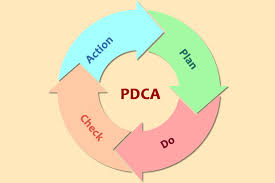
\includegraphics[width=0.48\linewidth]{../immagini/Ciclo_di_Deming.jpg}
		\caption{Rappresentazione del Ciclo di Deming}
	\end{center}
\end{figure}

	\chapter{Formazione}\label{Formazione}
\section{Processo di formazione}\label{FormazioneProcessoDiFormazione}
Tramite il processo di formazione si intendono fornire materiali e strumenti idonei a rendere il gruppo di lavoro qualificato allo sviluppo del prodotto software.
Questo processo consiste nelle seguenti attività:
\begin{enumerate}
	\item \textbf{Piano di formazione};
	\item \textbf{Ricerca del materiale};
	\item \textbf{Inizio della formazione}.
\end{enumerate}
\subsection{Piano di formazione}\label{FormazioneProcessoDiFormazionePianoDiFormazione}
In questa prima fase il gruppo di lavoro, assieme al \textit{Responsabile di progetto}, discuteranno e decideranno su quali siano le abilità principali e necessarie per diventare sviluppatori qualificati nell'ambito del prodotto software.
Questa decisione sarà basata sulle richieste proposte nel capitolato d'appalto del committente.
\subsection{Ricerca del materiale}\label{FormazioneProcessoDiFormazioneRicercaDelMateriale}
Una volta definito il piano da seguire si prosegue con la ricerca attiva del materiale da parte del gruppo.
Questo lavoro può essere svolto mediante tre macro-categorie:
\begin{itemize}
	\item \textbf{Libri}: quindi la ricerca tramite libri testuali, o digitali, contenenti nozioni sugli argomenti da imparare;
	\item \textbf{Azienda}: ovvero la richiesta di materiale specifico all'azienda proponente del software da sviluppare;
	\item \textbf{Internet}: quindi cercando su forum o siti specializzati informazioni pertinenti tutto ciò che riguarda il progetto.
\end{itemize}
\subsection{Inizio della formazione}\label{FormazioneProcessoDiFormazioneInizioDellaFormazione}
Raccolto il materiale adatto, il gruppo inizierà la propria formazione sia personale, sia collettiva nel caso qualche componente avesse problemi con alcuni concetti.

	% bibliography, glossary and index would go here.

\end{document}
